% !TeX root = ../../Book3.tex
% 纲要标题：## 第15章　Hodge 理论、Bochner 公式与分裂定理
% 纲要位置：几何学计划纲要.md，第 2704 行。
% 正文状态：初稿；尚未正式审核。

% 纲要内容开始
% 
% > 本章目标与证明范围：闭流形 Hodge 定理在全局椭圆工具之后完整证明。随后将 Weitzenböck 用于曲率消失；非紧分裂独立补齐截断、弱调和与 Busemann 的工具，不照搬紧情形积分。
% 
% 纲要内容结束

\chapter{Hodge 理论、Bochner 公式与分裂定理}
\label{g3:ch:15}
\BookChapterNumber{g3:ch:15}

\begin{chapterabstract}
	微分形式把上同调与椭圆方程联系起来。本章以 Hodge 星和形式伴随固定符号，由 Green 算子证明闭流形上的正合、余正合与调和分解，建立每个 de Rham 类的唯一调和代表及积分对偶。Weitzenböck 公式将调和条件转成联络能量与曲率作用的关系，给出正 Ricci 下的一阶消失和适当非负曲率条件下的平行性。转到非紧流形后，先用完备距离截断控制无穷远误差，辨明平方可积调和形式的范围，再建立连续弱次调和函数的最大值工具。最后由两侧 Busemann 函数完整证明 Cheeger--Gromoll 分裂。
\end{chapterabstract}

\begin{learninggoals}
	\begin{itemize}
		\item 计算不同次数的 Hodge 星、余微分与 Laplace 主符号，区分定向体积形式与正体积密度。
		\item 从 Green 恒等式得到 Hodge 分解，并为闭形式构造唯一调和代表及规范原像。
		\item 用星算子证明 de Rham 积分配对非退化，说明不可定向情形的系数改变。
		\item 推导一形式的 Ricci 项及函数 Bochner 公式，识别各阶消失结论的曲率假设。
		\item 构造完备流形上的紧支截断，估计环带误差，判断平方可积性与增长条件的作用。
		\item 通过调和替换证明连续弱次调和函数的强最大值原理，并把弱调和方程提升为光滑方程。
		\item 从一条测地直线构造两侧 Busemann 函数、平行单位梯度及整体等距乘积。
	\end{itemize}
\end{learninggoals}

在圆周上，一形式 \(\mathrm d\theta\) 闭合，却不是一个周期函数的微分：它沿圆周的积分为 \(2\pi\)，而周期函数的微分沿一周期积分为零。加入任意 \(\mathrm dF\) 不改变这个积分，却改变形式的点态系数。给定度量以后，能否从所有这些代表中选出一个最省能量的？对范数沿 \(\mathrm dF\) 方向作变分，出现的条件正是余闭方程 \(\delta\omega=0\)。它与原来的闭合条件共同给出 Hodge Laplace 方程。

\ProseParagraphBreak

椭圆理论保证闭流形上的这种选择存在而且唯一。几何信息随后进入：Weitzenböck 公式把形式 Laplace 写成联络 Laplace 加曲率项。调和形式若遇到非负的曲率作用，就必须平行；适当的严格正性再迫使它消失。圆球与平坦环面的差别由此体现为一阶上同调的差别。高阶形式看到的曲率作用更丰富，需要重新检验正性条件。

\ProseParagraphBreak

紧性在这条论证中并非可以省略的背景。在实直线上，函数 \(x\) 调和而不恒定；若把没有紧支的 \(x\) 直接代入整体能量恒等式，就会错误地得到其导数为零。非紧情形要先乘截断，留下的导数项由环带上的质量控制。一旦这些分析条件清楚，局部曲率公式又能用于整体几何：非负 Ricci 曲率下，一条在所有区间上都实现距离的测地直线将产生一个光滑调和函数，其梯度平行且长度为一，沿梯度流动便得到一个真实的直积因子。

\ProseParagraphBreak

本章使用第十一章的弱导数、迹与紧嵌入，第十二章的椭圆正则性和经典最大值原理，第十三章的 Fredholm 与 Green 算子，以及第十四章的弱 Dirichlet 求解。最后一节还接续第二章的完备性、七至八章的距离比较与 Busemann 函数。Hodge 与 Laplace 的进一步阅读可从 Jost 第3章\cite[第3章]{Jost2017}开始；曲率作用及 Bochner 方法可参阅 Petersen 第9章\cite[第9章]{Petersen2016}。

% !TeX root = ../../Book3.tex
% 纲要标题：### 15.1 微分形式上的椭圆结构
% 纲要位置：几何学计划纲要.md，第 2708 行。
% 正文状态：初稿；尚未正式审核。

% 纲要内容开始
% 
% * Hodge 星和形式伴随
% * Hodge Laplace 的主符号
% * 能量恒等式及调和条件
% * 定向与密度约定
% 
% 纲要内容结束

\section{微分形式上的椭圆结构}
\label{g3:sec:1501}

外微分记录形式的局部变化，却没有使用度量。度量提供第二个方向的算子：把外微分在积分配对中移到另一边，得到余微分。二者合成的 Laplace 算子既保留上同调的信息，又具有椭圆正则性。本节先把这些运算在形式上的含义、符号和定向条件写清楚，使后续的调和分解能够直接用于几何计算。

\subsection{Hodge 星和形式伴随}
\label{g3:subsec:1501:01}
设 \(M\) 为 \(n\) 维光滑黎曼流形，记 \(\Omega^k(M;\mathbb C)\) 为光滑复值 \(k\) 形式空间；实值空间记为 \(\Omega^k(M;\mathbb R)\)。在实正交余标架 \(e^1,\ldots,e^n\) 下，严格递增指标的 \(e^{i_1}\wedge\cdots\wedge e^{i_k}\) 构成形式丛的正交归一标架。诱导的 Hermitian 内积对第一变量线性，积分内积写成
\[
	(\alpha,\beta)=\int_M\langle\alpha,\beta\rangle_g\,\mu_g.
\]
这个定义只需要正体积密度。暂且给 \(M\) 选择定向，用 \(\operatorname{vol}_g\) 表示相应的体积形式。

\begin{definition}\label{g3:def:form-hodge-star}
	设 \(M\) 为定向光滑 \(n\) 维黎曼流形，\(0\le k\le n\)，\(\operatorname{vol}_g\) 为正定向体积形式。满足
	\begin{equation}\label{g3:eq:hodge-star-pairing}
		\alpha\wedge *\overline\beta
		=\langle\alpha,\beta\rangle_g\operatorname{vol}_g
		\qquad(\alpha,\beta\in\Lambda^k\mathrm T_x^*M\otimes\mathbb C)
	\end{equation}
	的复线性丛映射
	\[
		*:\Lambda^k\mathrm T^*M\otimes\mathbb C
		\longrightarrow\Lambda^{n-k}\mathrm T^*M\otimes\mathbb C
	\]
	称为 \term[Hodge xing]{Hodge 星算子}[Hodge star operator]。它是实形式上的星算子的复线性延拓，共轭显式写在式\eqref{g3:eq:hodge-star-pairing}中。
\end{definition}
\symidx{\(*\)：定向黎曼流形上的 Hodge 星算子}

这里确实存在唯一这样的映射。对正向正交余标架及递增指标 \(I\)，令 \(I^c\) 为补指标，并以 \(\epsilon(I,I^c)\) 表示排列 \((I,I^c)\) 的符号，则
\[
	*e^I=\epsilon(I,I^c)e^{I^c}.
\]
将这一公式与每个基向量外乘，正好得到定义中的配对，且外乘的非退化性保证唯一。定义本身与所选正向正交标架无关，因而局部公式拼成光滑丛映射。

\begin{proposition}\label{g3:prop:hodge-star-identities}
	在定向光滑 \(n\) 维黎曼流形上，令 \(\nabla\) 为 Levi-Civita 诱导的形式联络，\(X\) 为光滑向量场，\(0\le k\le n\)。Hodge 星算子保持逐点范数与内积，并满足
	\begin{equation}\label{g3:eq:hodge-star-square}
		**\alpha=(-1)^{k(n-k)}\alpha,\qquad
		\nabla_X(*\alpha)=*(\nabla_X\alpha)
		\quad(\alpha\in\Omega^k).
	\end{equation}
	若改变定向，星算子变为原来的负号。
\end{proposition}
\begin{proof}
	在正交外代数基中，星算子只把基向量带符号地换成补指标基，所以保持内积。再次取补指标，需要将长度为 \(k\) 与 \(n-k\) 的两组指标交换，符号为 \((-1)^{k(n-k)}\)。Levi--Civita 联络保持度量与定向体积形式；对定义等式求协变导数，用内积和外乘的乘积法则，再由配对的非退化性，得到与联络交换。反转定向使体积形式变号，定义中的星也随之变号。
\end{proof}

例如在标准定向的 \(\mathbb R^3\) 中，\(*\mathrm dx=\mathrm dy\wedge\mathrm dz\)、\(*(\mathrm dx\wedge\mathrm dy)=\mathrm dz\)。在定向曲面上，\(*e^1=e^2\)、\(*e^2=-e^1\)，因此一形式上的星平方为 \(-I\)。后一公式把一个余切方向转成与它正交的方向。

\ProseParagraphBreak

现在用积分定义反向的一阶算子。对内部紧支光滑形式，要求
\[
	(\mathrm d\alpha,\beta)=(\alpha,\delta\beta),
	\qquad \alpha\in\Omega_c^{k-1},\quad\beta\in\Omega_c^k.
\]
这里的 \(\delta=\mathrm d^*\) 称为\term[yuweifen]{余微分}[codifferential]。紧支条件消除了边界通量；在闭流形上可以直接对任意光滑形式使用这个配对。

\begin{proposition}\label{g3:prop:codifferential-star}
	设 \(M\) 为光滑 \(n\ge1\) 维黎曼流形，\(\delta\) 为外微分相对于诱导形式内积及正体积密度的形式伴随。在局部正交标架中，
	\begin{equation}\label{g3:eq:form-covariant-d-delta}
		\mathrm d=\sum_i e^i\wedge\nabla_{e_i},
		\qquad
		\delta=-\sum_i\iota_{e_i}\nabla_{e_i}.
	\end{equation}
	若 \(M\) 定向，则在 \(k\) 形式上
	\begin{equation}\label{g3:eq:codifferential-star}
		\delta=(-1)^{n(k+1)+1}*\mathrm d*.
	\end{equation}
\symidx{\(\delta=\mathrm d^*\)：微分形式上的余微分}
	在零形式上取 \(\delta=0\)，在最高次形式上取 \(\mathrm d=0\)；各次数均有 \(\delta^2=0\)。
\end{proposition}
\begin{proof}
	无挠性使外微分等于协变导数的交替化，给出第一式。外乘 \(e^i\) 的逐点伴随是收缩 \(\iota_{e_i}\)。在任一点取该点协变导数为零的正交标架，将导数分部积分，形式伴随在该点就是 \(-\sum_i\iota_{e_i}\nabla_{e_i}\)。所写表达式是协变导数的张量收缩，与正交标架无关，因此在整个流形上成立。

	定向情形还可直接看出星公式的符号。对紧支的 \((k-1)\) 形式 \(\alpha\) 与 \(k\) 形式 \(\beta\)，Stokes 公式及乘积法则给出
	\[
		\int_M\mathrm d\alpha\wedge *\overline\beta
		=(-1)^k\int_M\alpha\wedge\mathrm d*\overline\beta.
	\]
	所以 \(*\delta\beta=(-1)^k\mathrm d*\beta\)。用式\eqref{g3:eq:hodge-star-square}消去左边的星，所得指数与 \(n(k+1)+1\) 相差偶数，得到式\eqref{g3:eq:codifferential-star}。最后对任意紧支测试形式 \(\eta\)，有
	\((\delta^2\beta,\eta)=(\beta,\mathrm d^2\eta)=0\)，故 \(\delta^2\beta=0\)。这一局部结论不需要紧性或定向。
\end{proof}

把一形式写为 \(\alpha=X^\flat\)，协变表达式给出 \(\delta\alpha=-\operatorname{div}X\)。在 Euclid 平面上，若 \(\alpha=a\,\mathrm dx+b\,\mathrm dy\)，则
\[
	\delta\alpha=-(\partial_xa+\partial_yb),\qquad
	\delta(f\,\mathrm dx\wedge\mathrm dy)
	=\partial_yf\,\mathrm dx-\partial_xf\,\mathrm dy.
\]
这些计算同时核对了余微分和本书非负 Laplace 算子的符号。

\subsection{Hodge Laplace 的主符号}
\label{g3:subsec:1501:02}
闭形式的条件是 \(\mathrm d\omega=0\)，而与所有正合形式正交的条件是 \(\delta\omega=0\)。把这两个方程的平方能量合在一起，定义 \(k\) 形式上的\term[Hodge Laplace suanzi]{Hodge Laplace 算子}[Hodge Laplacian]
\[
	\Delta_k=\mathrm d\delta+\delta\mathrm d.
\]
次数下标在对象清楚时省略。对函数，\(\Delta_0=\delta\mathrm d=-\operatorname{div}\operatorname{grad}\)，与前文约定一致。

\begin{proposition}\label{g3:prop:hodge-laplacian-symbol}
	设 \(M\) 为光滑 \(n\ge1\) 维黎曼流形，\(0\le k\le n\)。记 \(\delta=\mathrm d^*\) 为形式伴随，\(\Delta_k=\mathrm d\delta+\delta\mathrm d\) 为 \(k\) 次形式上的 Hodge Laplace 算子。则 \(\Delta_k\) 为光滑二阶椭圆算子，且沿用 \(\mathrm D_j=-\mathrm i\partial_j\) 的主符号约定时，
	\begin{equation}\label{g3:eq:hodge-symbol}
		\sigma_1(\mathrm d)(x,\xi)=\mathrm i\,\varepsilon_\xi,\qquad
		\sigma_1(\delta)(x,\xi)=-\mathrm i\,\iota_{\xi^\sharp},\qquad
		\sigma_2(\Delta_k)(x,\xi)=|\xi|_g^2I.
	\end{equation}
	这里 \(\xi\) 是实余切向量，\(\varepsilon_\xi\alpha=\xi\wedge\alpha\)。
\end{proposition}
\symidx{\(\Delta_k=\mathrm d\delta+\delta\mathrm d\)：\(k\) 次形式上的 Hodge Laplace 算子}
\begin{proof}
	在一点取正交标架，式\eqref{g3:eq:form-covariant-d-delta}的最高阶项给出前两个符号。对任意形式，收缩乘积法则为
	\[
		\iota_{\xi^\sharp}(\xi\wedge\alpha)
		=|\xi|^2\alpha-\xi\wedge\iota_{\xi^\sharp}\alpha.
	\]
	因此两种复合符号之和等于 \(|\xi|^2I\)，非零 \(\xi\) 时可逆。这也直接恢复了\cref{g3:lem:wedge-contraction-symbol}在实余切方向的计算；联络和度量的导数只进入较低阶项。
\end{proof}

同一个外乘收缩恒等式还说明 de Rham 符号序列正合：若 \(\xi\wedge\alpha=0\)，则
\[
	\alpha=\xi\wedge\bigl(|\xi|^{-2}\iota_{\xi^\sharp}\alpha\bigr).
\]
所以第十三章的一般椭圆复形理论确实适用于形式。这里的椭圆性是局部性质，在非紧流形上同样成立；有限维核和整体分解还需要下一节所列的紧性。

\subsection{能量恒等式及调和条件}
\label{g3:subsec:1501:03}
\begin{proposition}\label{g3:prop:form-hodge-energy}
	设 \(M\) 为无边界光滑黎曼流形，\(\omega,\eta\) 为光滑 \(k\) 形式。记 \(\delta=\mathrm d^*\) 为形式伴随，\(\Delta_k=\mathrm d\delta+\delta\mathrm d\) 为 \(k\) 次形式上的 Hodge Laplace 算子。括号取体积密度及形式内积确定的 \(L^2\) 配对。若 \(M\) 紧，或两形式至少有一个紧支，则
	\begin{equation}\label{g3:eq:form-hodge-energy}
		(\Delta_k\omega,\eta)
		=(\mathrm d\omega,\mathrm d\eta)+(\delta\omega,\delta\eta)
		=(\omega,\Delta_k\eta).
	\end{equation}
	特别地，在闭黎曼流形上，
	\[
		\Delta_k\omega=0
		\quad\Longleftrightarrow\quad
		\mathrm d\omega=0,\quad\delta\omega=0.
	\]
	此结论对实值与复值形式都成立，且不要求定向。
\end{proposition}
\begin{proof}
	对 \(\mathrm d\delta\) 与 \(\delta\mathrm d\) 分别用形式伴随定义，即得两项能量及对称性。取 \(\eta=\omega\)，在紧流形上有
	\[
		(\Delta_k\omega,\omega)=\|\mathrm d\omega\|_2^2+\|\delta\omega\|_2^2.
	\]
	左侧为零时，两个非负项都为零；光滑性将几乎处处为零提升为处处为零。反方向直接代入 \(\Delta_k\) 的定义。
\end{proof}

满足 \(\Delta_k\omega=0\) 的光滑形式称为\term[tiaohe xingshi]{调和形式}[harmonic form]，其空间记为 \(\mathcal H_g^k(M)\)。在闭流形上，命题把这个二阶方程换成闭合与余闭合两个一阶条件。非紧情形则需保留积分条件：在 \(\mathbb R\) 上，函数 \(x\) 满足 \(\Delta x=0\)，但 \(\mathrm dx\ne0\)；它不能直接代入一个要求紧支或有限能量的整体积分论证。

\begin{proposition}\label{g3:prop:hodge-star-commutes}
	设 \(M\) 为定向光滑 \(n\) 维黎曼流形。记 \(\delta=\mathrm d^*\) 为形式伴随，\(\Delta_k=\mathrm d\delta+\delta\mathrm d\) 为 \(k\) 次形式上的 Hodge Laplace 算子。以 \(*\) 为 Hodge 星，对 \(0\le k\le n\) 的光滑 \(k\) 形式 \(\alpha\)，有
	\begin{align*}
		\mathrm d*\alpha&=(-1)^k*\delta\alpha,&
		\delta*\alpha&=(-1)^{k+1}*\mathrm d\alpha,\\
		\Delta_{n-k}*\alpha&=*\Delta_k\alpha.
	\end{align*}
	此外，在任意光滑黎曼流形上有 \(\mathrm d\Delta=\Delta\mathrm d\)、\(\delta\Delta=\Delta\delta\)，各式按相应次数解释。
\end{proposition}
\begin{proof}
	前两个等式由式\eqref{g3:eq:codifferential-star}及星的平方公式得到。分别将它们用于 \(\mathrm d\delta*\alpha\) 与 \(\delta\mathrm d*\alpha\)，两次出现的次数符号抵消，得到星与 Laplace 的交换。余下两式只需展开并使用 \(\mathrm d^2=\delta^2=0\)；例如 \(\mathrm d\Delta=\mathrm d\delta\mathrm d=\Delta\mathrm d\)。
\end{proof}

因而在定向闭流形上，星将 \(k\) 次调和形式同构地送到 \(n-k\) 次调和形式。这个算子将成为下一节积分配对非退化的具体见证。

\subsection{定向与密度约定}
\label{g3:subsec:1501:04}
星算子使用定向体积形式，而 \((\cdot,\cdot)\)、\(\delta\) 和 \(\Delta\) 使用正体积密度。反转定向时，式\eqref{g3:eq:codifferential-star}中的两个星同时变号，\(\delta\) 不变。因此在不可定向流形上，可以在每个坐标邻域选择定向并计算 \(\delta,\Delta\)，重叠处所得算子相同。式\eqref{g3:eq:form-covariant-d-delta}则直接给出了不依赖定向的整体表达式。

\ProseParagraphBreak

若仍要保留星，需记录局部定向的符号。记 \(o_M\) 为\term[dingxiang xiancong]{定向线丛}[orientation line bundle]：在每个有定向的坐标邻域取一个单位生成元，换向的重叠处以 \(-1\) 为过渡函数，同向处以 \(1\) 为过渡函数。这些局部常值过渡函数定义平坦度量实线丛，且 \(o_M\otimes o_M\) 有自然的平凡化。记 \(\Omega^k(M;o_M)\) 为取值于它的形式；局部对系数作外微分得到全局算子 \(\mathrm d_o\)，因为过渡函数的导数为零。

\begin{proposition}\label{g3:prop:twisted-hodge-star}
	设 \(M\) 为任意光滑 \(n\) 维黎曼流形。记 \(o_M\) 为带自然平坦联络的定向线丛。局部 Hodge 星算子定义整体映射
	\[
		*:\Omega^k(M;\mathbb R)\longrightarrow\Omega^{n-k}(M;o_M),
		\qquad
		*:\Omega^k(M;o_M)\longrightarrow\Omega^{n-k}(M;\mathbb R).
	\]
	它们在 \(k\) 次形式上的复合为 \((-1)^{k(n-k)}I\)，并将普通与定向线丛值的 Laplace 算子交织。普通形式与互补次数的定向线丛值形式的外积是可积分的顶次密度。
\end{proposition}
\begin{proof}
	换向时，局部星与 \(o_M\) 的单位生成元都变号，故两者的乘积不变。反方向使用 \(o_M^{\otimes2}\) 的自然平凡化，得到第二个映射。所有平方、伴随和交换公式都是局部恒等式，而线丛过渡函数局部常值，所以前面的计算逐图适用并相容。

	最后，顶次形式在反向坐标变换下的符号由定向线丛因子抵消；局部表达式因而按 Jacobian 的绝对值变换。这正是密度的变换规则。用单位分解积分，结果与图册及局部定向选择无关；紧支的定向线丛值 \((n-1)\) 形式也满足 Stokes 公式，逐图积分后单位分解的导数项相消。
\end{proof}

当 \(M\) 可定向并选定定向时，\(o_M\) 获得一个平行单位截面，以上两种形式便可识别。没有这种选择时，普通顶次形式与顶次密度仍是不同对象；下一节的对偶结论将相应地使用定向线丛系数。
% 纲要条目排为编号小节标题，并进入目录与书签；说明段仍保留于纲要注释中。

% !TeX root = ../../Book3.tex
% 纲要标题：### 15.2 Hodge 定理的证明
% 纲要位置：几何学计划纲要.md，第 2715 行。
% 正文状态：初稿；尚未正式审核。

% 纲要内容开始
% 
% * 正合、余正合及调和分解
% * 每个 de Rham 类的调和代表
% * 唯一性、有限维性和自然配对
% * Poincaré 对偶的解析再解释
% 
% 纲要内容结束

\section{Hodge 定理的证明}
\label{g3:sec:1502}

一个闭形式有许多相差正合形式的代表。要从中作出有几何意义的选择，可以要求代表正交于所有正合方向，也就是同时满足余闭条件。上一节把这两个一阶条件合成了椭圆方程；现在借助第十三章已经建立的 Green 算子，证明这样的代表总能选出，并说明它与积分配对的关系。以下“闭流形”指紧致、无边界的光滑流形。

\subsection{正合、余正合及调和分解}
\label{g3:subsec:1502:01}
固定闭黎曼流形 \(M\)，暂取复值形式。由\cref{g3:prop:hodge-laplacian-symbol,g3:prop:form-hodge-energy}，\(\Delta_k\) 是形式自伴、非负的二阶椭圆算子。因此\cref{g3:thm:elliptic-fredholm,g3:thm:elliptic-green-general}适用：其核 \(\mathcal H_g^k\) 有限维且光滑，存在 \(L^2\) 正交投影 \(\Pi_k\) 及 Green 算子 \(G_k\)，满足
\begin{equation}\label{g3:eq:form-green-identities}
	\Delta_kG_k=I-\Pi_k,\qquad
	G_k\Delta_k=I-\Pi_k,\qquad
	G_k\Pi_k=\Pi_kG_k=0.
\end{equation}
第二式的定义域为 \(H^2\)，而 \(G_k:H^s\to H^{s+2}\) 对整数 \(s\ge0\) 有界；特别地，它把光滑形式送到光滑形式。

\begin{theorem}[闭流形上的 Hodge 分解]\label{g3:thm:closed-hodge-decomposition}
	设 \(M\) 为闭的 \(n\ge1\) 维黎曼流形，\(0\le k\le n\)。则有 \(L^2\) 正交直和
	\begin{equation}\label{g3:eq:closed-form-hodge-decomposition}
		\Omega^k(M;\mathbb C)
		=\mathcal H_g^k
		\oplus\mathrm d\Omega^{k-1}(M;\mathbb C)
		\oplus\delta\Omega^{k+1}(M;\mathbb C).
	\end{equation}
	端点处不存在的形式空间取零。任意 \(\omega\) 的三个分量为
	\begin{equation}\label{g3:eq:form-hodge-components}
		\omega=\Pi_k\omega
		+\mathrm d(\delta G_k\omega)
		+\delta(\mathrm dG_k\omega).
	\end{equation}
	在 \(L^2\) 中还成立闭子空间的正交直和
	\[
		L^2(\Lambda^k)
		=\mathcal H_g^k
		\oplus\mathrm dH^1(\Lambda^{k-1})
		\oplus\delta H^1(\Lambda^{k+1}).
	\]
	同样结论适用于实值形式。
\end{theorem}
\begin{proof}
	由式\eqref{g3:eq:form-green-identities}，展开 \(\Delta_kG_k\) 便得到式\eqref{g3:eq:form-hodge-components}。若 \(\alpha,\beta,h\) 光滑且 \(h\) 调和，则
	\[
		(\mathrm d\alpha,\delta\beta)
		=(\mathrm d^2\alpha,\beta)=0,\qquad
		(\mathrm d\alpha,h)=(\alpha,\delta h)=0,\qquad
		(\delta\beta,h)=(\beta,\mathrm dh)=0.
	\]
	所以所得分量两两正交，因而唯一。分量的原像 \(\alpha,\beta\) 可以改变；唯一性说的是 \(\mathrm d\alpha,\delta\beta,h\)。

	为取得 \(L^2\) 结论，记 \(E_k=\mathrm d\delta G_k\)、\(C_k=\delta\mathrm dG_k\)。Green 算子的两阶增益使二者在 \(L^2\) 上有界。光滑分解证明了 \(\Pi_k,E_k,C_k\) 在稠密的光滑子空间上是互相正交的投影；取极限后在全 \(L^2\) 上仍然如此，故其像闭。

	由 \(\delta G_k:L^2\to H^1\)，有 \(\operatorname{ran}E_k\subset\mathrm dH^1\)。反过来，若 \(\alpha\in H^1\)，以光滑 \(\alpha_j\) 在 \(H^1\) 中逼近，则
	\(E_k\mathrm d\alpha_j=\mathrm d\alpha_j\) 收敛为 \(E_k\mathrm d\alpha=\mathrm d\alpha\)，故两像相等。余正合像同理。这也是\cref{g3:thm:elliptic-complex-hodge-decomposition}在外微分复形上的具体实现。最后，\(\Delta_k\) 具有实系数；共轭保持核与正交补，规范解的唯一性使 \(G_k\)、\(\Pi_k\) 与共轭交换。因此对实形式得到的全部分量仍为实形式。
\end{proof}

正合部分测量能够由低一次形式的外微分产生的变化，余正合部分则与闭形式正交。这个分解还给出求解条件：
\[
	\Delta_k u=f\text{ 可解}
	\quad\Longleftrightarrow\quad
	(f,h)=0\quad\text{对所有 }h\in\mathcal H_g^k.
\]
满足正交条件时，\(G_kf\) 是唯一正交于调和核的解。于是调和空间同时承担上同调代表与椭圆方程可解障碍两种职责。

\subsection{每个 de Rham 类的调和代表}
\label{g3:subsec:1502:02}
对 \(\mathbb F=\mathbb R\) 或 \(\mathbb C\)，回忆光滑 de Rham 上同调的定义：
\[
	H_{\mathrm{dR}}^k(M;\mathbb F)
	=\frac{\ker(\mathrm d:\Omega^k\to\Omega^{k+1})}
	{\mathrm d\Omega^{k-1}}.
\]
分子中的形式闭合，等价关系要求差为一个光滑形式的外微分。这个定义没有使用黎曼度量。

\begin{theorem}[Hodge 定理]\label{g3:thm:hodge-de-rham}
	设 \(M\) 为闭的 \(n\ge1\) 维黎曼流形，\(0\le k\le n\)，\(\mathbb F=\mathbb R\) 或 \(\mathbb C\)。映射
	\[
		\mathcal H_g^k(M;\mathbb F)\longrightarrow
		H_{\mathrm{dR}}^k(M;\mathbb F),\qquad h\longmapsto[h]
	\]
	为线性同构。具体地，若 \(\mathrm d\omega=0\)，则
	\begin{equation}\label{g3:eq:hodge-closed-representative}
		\omega=\Pi_k\omega+\mathrm d(\delta G_k\omega).
	\end{equation}
	因此每个上同调类有唯一调和代表，且上同调有限维；这里不要求 \(M\) 定向。
\end{theorem}
\begin{proof}
	调和形式闭合，故映射有定义。设 \(\omega=h+\mathrm d\alpha+\delta\beta\) 为上一分解，且 \(\mathrm d\omega=0\)。用伴随公式与正交性，
	\[
		\|\delta\beta\|_2^2
		=(\omega,\delta\beta)=(\mathrm d\omega,\beta)=0.
	\]
	于是余正合部分为零，\(\omega\) 与 \(h=\Pi_k\omega\) 相差正合形式，给出存在性及式\eqref{g3:eq:hodge-closed-representative}。若两个调和代表之差为 \(h=\mathrm d\alpha\)，则
	\(\|h\|_2^2=(h,\mathrm d\alpha)=(\delta h,\alpha)=0\)，故二者相同。核的有限维性随即给出上同调的有限维性。全部步骤在实形式空间内也成立。
\end{proof}

同一个证明说明如何为正合形式选择原像。若 \(k\ge1\)、\(\omega\) 光滑且正合，则
\[
	\alpha_0=\delta G_k\omega,\qquad
	\mathrm d\alpha_0=\omega,\qquad
	\delta\alpha_0=0,\qquad \Pi_{k-1}\alpha_0=0.
\]
最后一式来自 \(\alpha_0\) 是余正合形式。任意其他原像为 \(\alpha_0+\zeta\)，其中 \(\mathrm d\zeta=0\)；而
\((\alpha_0,\zeta)=(G_k\omega,\mathrm d\zeta)=0\)。
所以 \(\alpha_0\) 是唯一范数最小的光滑原像，且
\[
	\|\alpha_0\|_{H^{s+1}}\le C_s\|\omega\|_{H^s}
	\qquad(s=0,1,\ldots).
\]
这把“存在原像”加强成了带有规范与估计的求解。

\begin{example}\label{g3:exm:hodge-variable-circle}
	在 \(\mathbb R/2\pi\mathbb Z\) 上取 \(g=a(\theta)^2\mathrm d\theta^2\)，其中 \(a>0\) 光滑且周期。令 \(L=\int_0^{2\pi}a(\theta)\,\mathrm d\theta\)。每个一形式 \(f(\theta)\,\mathrm d\theta\) 都闭合，而
	\[
		*\bigl(f\,\mathrm d\theta\bigr)=\frac f a,\qquad
		\delta(f\,\mathrm d\theta)
		=-\frac1a\,\frac{\mathrm d}{\mathrm d\theta}\left(\frac f a\right).
	\]
	故调和一形式恰为 \(c\,a(\theta)\,\mathrm d\theta\)。给定 \(\omega=f\,\mathrm d\theta\)，取
	\[
		c=\frac1L\int_0^{2\pi}f(\theta)\,\mathrm d\theta,\qquad
		F(\theta)=\int_0^\theta(f(s)-c\,a(s))\,\mathrm ds.
	\]
	被积函数在一周期的积分为零，故 \(F\) 是周期光滑函数，且
	\(\omega=c\,a\,\mathrm d\theta+\mathrm dF\)。
	上同调类由周期积分决定，调和代表的具体系数却随度量改变。
\end{example}

\subsection{唯一性、有限维性和自然配对}
\label{g3:subsec:1502:03}
设 \(c\) 是一个 de Rham 类，\(h_c\) 为其调和代表。任何光滑代表都可写成 \(h_c+\mathrm d\alpha\)，因而
\[
	\|h_c+\mathrm d\alpha\|_2^2
	=\|h_c\|_2^2+\|\mathrm d\alpha\|_2^2.
\]
所以调和代表是给定上同调类中唯一的最小 \(L^2\) 范数代表。另一方面，沿正合方向作一阶变分，最小值条件就是 \((h_c,\mathrm d\alpha)=0\)，即 \(\delta h_c=0\)。这解释了余闭条件为何能消除代表选择中的自由度。

\ProseParagraphBreak

由此在上同调上得到正定配对
\begin{equation}\label{g3:eq:hodge-inner-product-cohomology}
	\langle c_1,c_2\rangle_g=(h_{c_1},h_{c_2})_{L^2}.
\end{equation}
实系数时它是实内积，复系数时是第一变量线性的 Hermitian 内积。定义不依赖代表元，但依赖度量；上同调本身和维数 \(b_k=\dim H_{\mathrm{dR}}^k(M;\mathbb R)\) 则不依赖度量。

\begin{proposition}\label{g3:prop:hodge-naturality}
	设 \(M,N\) 为闭黎曼流形，\(F:N\to M\) 光滑。以两端的 Hodge 同构识别上同调后，拉回映射由
	\[
		\mathcal H_g^k(M)\longrightarrow\mathcal H_h^k(N),
		\qquad\omega\longmapsto\Pi_{N,k}F^*\omega
	\]
	表示。这些映射与恒等及复合相容。若 \(F\) 为黎曼等距微分同胚，则 \(F^*\omega\) 本身调和，无需再次投影。
	同一闭流形上的两个度量 \(g_0,g_1\) 给出同构
	\[
		\mathcal H_{g_0}^k\longrightarrow\mathcal H_{g_1}^k,
		\qquad h\longmapsto\Pi_{g_1,k}h,
	\]
	其逆为另一方向的调和投影。
\end{proposition}
\begin{proof}
	拉回与外微分交换，故保持闭形式与正合形式。Hodge 定理说明投影后的形式仍代表同一拉回类，且这个类的调和代表唯一。对复合映射，任何中途投影只使闭形式改变一个正合项；再次拉回仍是正合项，最终投影消去它。这证明复合相容，恒等情形直接成立。

	等距微分同胚保持诱导形式内积与体积密度。将形式伴随等式拉回，得到 \(F^*\delta_M=\delta_NF^*\)，于是它也与 Laplace 交换。度量改变的两张映射则都保持原上同调类；先后应用两次，得到与原形式同类的调和形式，由唯一性即为原形式。
\end{proof}

调和代表还可用于计算上同调乘积，但取外积后通常需要再次投影。若 \(h_1,h_2\) 调和，它们闭合，所以
\[
	h_1\mathbin{\smile_g}h_2=\Pi(h_1\wedge h_2)
\]
代表原来两类的外积。这个乘法在调和空间上结合、分次交换，因为对应的 de Rham 类具有这些性质，调和代表又唯一。

\begin{example}\label{g3:exm:harmonic-wedge-not-harmonic}
	在二维环面 \((\mathbb R/2\pi\mathbb Z)^2\) 上取
	\(g=e^{2\varphi(x,y)}(\mathrm dx^2+\mathrm dy^2)\)，其中 \(\varphi\) 光滑、周期且非常数。正交余标架为 \(e^\varphi\mathrm dx,e^\varphi\mathrm dy\)，故
	\[
		*\mathrm dx=\mathrm dy,\qquad *\mathrm dy=-\mathrm dx,\qquad
		*(\mathrm dx\wedge\mathrm dy)=e^{-2\varphi}.
	\]
	一形式 \(\mathrm dx,\mathrm dy\) 均闭且余闭，所以调和；它们的外积却不余闭，因为
	\(\mathrm d(e^{-2\varphi})\not\equiv0\)。
	调和顶次形式为体积形式的常数倍，故这个外积的调和代表是
	\[
		\Pi_2(\mathrm dx\wedge\mathrm dy)
		=\frac{4\pi^2}{\operatorname{Vol}_g(M)}\operatorname{vol}_g.
	\]
	系数由积分相等确定，也可直接用顶次调和空间上的正交投影计算。调和条件选出了每个类的代表，却不使这些代表在普通外积下封闭。
\end{example}

\subsection{Poincaré 对偶的解析再解释}
\label{g3:subsec:1502:04}
Hodge 内积依赖度量。另一个配对来自互补次数形式的外积积分：
\[
	\mathcal I([\alpha],[\beta])=\int_M\alpha\wedge\beta.
\]
它只需要闭流形的定向。若用 \(\alpha+\mathrm d\eta\) 替换闭形式 \(\alpha\)，增加的积分是 \(\int_M\mathrm d(\eta\wedge\beta)=0\)；替换 \(\beta\) 同理。因此它确实定义在上同调类上。

\begin{theorem}\label{g3:thm:hodge-poincare-duality}
	设 \(M\) 为闭、定向的 \(n\ge1\) 维光滑流形，\(\mathbb F=\mathbb R\) 或 \(\mathbb C\)。对每个 \(k\)，双线性配对
	\begin{equation}\label{g3:eq:de-rham-duality-pairing}
		H_{\mathrm{dR}}^k(M;\mathbb F)
		\times H_{\mathrm{dR}}^{n-k}(M;\mathbb F)
		\longrightarrow\mathbb F,\qquad
		([\alpha],[\beta])\longmapsto\int_M\alpha\wedge\beta
	\end{equation}
	非退化，因而给出
	\[
		H_{\mathrm{dR}}^k(M;\mathbb F)
		\cong \bigl(H_{\mathrm{dR}}^{n-k}(M;\mathbb F)\bigr)^*.
	\]
	配对与所选黎曼度量无关；任取一个度量，星算子在调和形式间给出依赖这个度量的同构 \(\mathcal H_g^k\cong\mathcal H_g^{n-k}\)。
\end{theorem}
\begin{proof}
	良定义已经由 Stokes 公式得到。选择一个黎曼度量，并取一个非零类的调和代表 \(h\)。\cref{g3:prop:hodge-star-commutes}说明 \(*\overline h\) 调和，特别地闭合；实系数时共轭可以省略。于是
	\[
		\int_M h\wedge *\overline h
		=\|h\|_2^2>0.
	\]
	所以左核为零。交换两个次数，用同一论证得到右核也为零；Hodge 定理已给出两空间有限维，双边非退化于是给出到线性对偶的同构。积分配对的定义没有用度量；星所给的具体代表和同构则使用了度量。
\end{proof}

这就是 de Rham 形式的 Poincaré 对偶。它的解析证明把一个非零类变成调和形式，再用星构造一个与它积分不为零的互补次数类。尤其 \(b_k=b_{n-k}\)。若 \(M\) 连通，则调和函数为常数，故 \(b_0=b_n=1\)；若 \(n\) 为奇数，交替和 \(\sum_k(-1)^k b_k\) 中互补次数两两抵消。若 \(n=2m\)，中间次数的配对满足
\[
	\mathcal I(c_2,c_1)=(-1)^m\mathcal I(c_1,c_2).
\]
当 \(m\) 为奇数时，它是非退化交替型，所以 \(b_m\) 为偶数：在实基中交替矩阵 \(A\) 满足 \(A^{\mathsf T}=-A\)，奇数阶时其行列式必为零。

\ProseParagraphBreak

不可定向流形使用上一节的定向线丛。其平坦微分 \(\mathrm d_o\) 的主符号仍为 \(\mathrm i\varepsilon_\xi\)，形式内积与正密度给出伴随 \(\delta_o\)。因此第十三章的椭圆复形分解适用于这个秩一系数复形，证明每个 \(H_{\mathrm{dR}}^j(M;o_M)\) 类也有唯一调和代表。由\cref{g3:prop:twisted-hodge-star}，普通与定向线丛值调和形式被星互相对应，重复前面的正范数论证便得到非退化配对
\begin{equation}\label{g3:eq:twisted-poincare-pairing}
	H_{\mathrm{dR}}^k(M;\mathbb R)
	\times H_{\mathrm{dR}}^{n-k}(M;o_M)
	\longrightarrow\mathbb R.
\end{equation}
这里顶次定向线丛值形式作为密度积分，因而不需选择整体定向。

\ProseParagraphBreak

例如，连通闭流形上 \(H_{\mathrm{dR}}^n(M;o_M)\cong\mathbb R\)，对应常数函数。若流形不可定向，则普通的 \(H_{\mathrm{dR}}^n(M;\mathbb R)=0\)：经星，这个空间对应定向线丛上的调和零形式；能量恒等式使这样的截面平行。非零平行截面处处不为零，归一化以后会选择一个整体定向，矛盾。于是定向条件在最高次上同调中留下了可直接检测的差别。
% 纲要条目排为编号小节标题，并进入目录与书签；说明段仍保留于纲要注释中。

% !TeX root = ../../Book3.tex
% 纲要标题：### 15.3 Weitzenböck 公式与 Bochner 方法
% 纲要位置：几何学计划纲要.md，第 2722 行。
% 正文状态：初稿；尚未正式审核。

% 纲要内容开始
% 
% * 联络 Laplace 和曲率作用
% * 一形式上的 Ricci 项
% * 正 Ricci 下的消失
% * 调和形式的平行性与维数界
% * 高阶形式的曲率项与曲率算子
% 
% 纲要内容结束

\section{Weitzenböck 公式与 Bochner 方法}
\label{g3:sec:1503}

Hodge 定理把上同调类交给调和形式来表示；曲率条件若能限制这些形式，就能限制流形的拓扑。关键是把形式 Laplace 算子与联络产生的二阶算子比较。两者具有相同主部，其差是曲率的零阶作用，这就是\term[Weitzenbock gongshi]{Weitzenböck 公式}[Weitzenböck formula]。\footnote{Roland Weitzenböck（1885--1955），奥地利数学家，长期任教于荷兰，研究不变量理论与微分几何。}

\ProseParagraphBreak

将这个恒等式与形式自身配对，得到范数的微分公式或积分公式。\term[Bochner fangfa]{Bochner 方法}[Bochner method]利用其中非负项之和为零，推出平行性或消失。\footnote{Salomon Bochner（1899--1982），美国数学家，出生于今波兰，研究调和分析、概率论与几何分析。}本节始终使用非负号约定
\(\Delta f=-\operatorname{div}\nabla f\)，并沿用
\(\mathrm{Rm}(X,Y,Z,W)=g(R(X,Y)W,Z)\)。固定度量后简记
\(\mathcal H^q(M)=\mathcal H_g^q(M)\)，并记
\(b_q(M)=\dim_{\mathbb R}H_{\mathrm{dR}}^q(M;\mathbb R)\)。
局部恒等式不要求紧性；将它积分为消失结论时，才明确假设流形是闭流形。

\subsection{联络 Laplace 和曲率作用}
\label{g3:subsec:1503:01}
设 \(E\to M\) 为带度量及相容联络的实或复向量丛。联络
\(\nabla:\Gamma(E)\to\Gamma(\mathrm T^*M\otimes E)\)
有形式伴随 \(\nabla^*\)，相应的\term[lianluo laplace suanzi]{联络 Laplace 算子}[connection Laplacian]为
\(\nabla^*\nabla\)。在正交单位标架中，
\begin{equation}\label{g3:eq:rough-laplacian-local}
	\nabla^*\nabla s
	=-\sum_i\bigl(\nabla_{e_i}\nabla_{e_i}s
	                  -\nabla_{\nabla_{e_i}e_i}s\bigr).
\end{equation}
第二项扣除了求导方向自身的变化，因而右侧是协变 Hessian 的负迹，与标架无关。对紧支截面 \(s,t\)，度量相容性和散度定理给出
\[
	(\nabla^*\nabla s,t)_{L^2}=(\nabla s,\nabla t)_{L^2}.
\]
这里及以下的复内积均对第一变量线性，积分使用黎曼体积密度，因而不需要定向。

\begin{lemma}\label{g3:lem:connection-norm-laplacian}
	设 \(M\) 为光滑无边界黎曼流形，\(E\) 带相容联络，\(s\) 为光滑截面。则逐点有
	\[
		\frac12\Delta|s|^2
		=\operatorname{Re}\langle\nabla^*\nabla s,s\rangle-|\nabla s|^2.
	\]
\end{lemma}
\begin{proof}
	在给定点取 \(\nabla_{e_i}e_j=0\) 的局部正交标架。度量相容性给出
	\(e_i|s|^2=2\operatorname{Re}\langle\nabla_{e_i}s,s\rangle\)，再求一次导数得
	\[
		e_i e_i|s|^2
		=2\operatorname{Re}\langle\nabla_{e_i}\nabla_{e_i}s,s\rangle
		 +2|\nabla_{e_i}s|^2.
	\]
	取负迹并用式\eqref{g3:eq:rough-laplacian-local}即可。一般标架中的联络修正项恰好恢复 Hessian 的迹。
\end{proof}

现在令 \(E=\Lambda^q\mathrm T^*M\)，联络由 Levi-Civita 联络诱导。记
\[
	\varepsilon_i\omega=e^i\wedge\omega,\qquad
	\iota_i\omega=\iota_{e_i}\omega,\qquad
	R^\Lambda(X,Y)=[\nabla_X,\nabla_Y]-\nabla_{[X,Y]}.
\]
诱导曲率对协变槽的作用为
\begin{equation}\label{g3:eq:curvature-action-on-forms}
	(R^\Lambda(X,Y)\omega)(Z_1,\ldots,Z_q)
	=-\sum_{a=1}^q
	\omega(Z_1,\ldots,R(X,Y)Z_a,\ldots,Z_q).
\end{equation}
此式可由协变导数的乘法法则求两次交换子得到：对标量配对的交换子扣除 Lie 括号后为零，故输入向量上的曲率作用移到形式一侧时带负号。

\begin{theorem}[Weitzenböck 公式]\label{g3:thm:weitzenbock-forms}
	设 \(M^n\) 为光滑无边界黎曼流形，\(0\le q\le n\)，
	\(\Delta_q=\mathrm d\delta+\delta\mathrm d\) 作用于实或复 \(q\) 形式。则
	\begin{equation}\label{g3:eq:weitzenbock-forms}
		\Delta_q=\nabla^*\nabla+\mathcal R_q,\qquad
		\mathcal R_q=-\sum_{i,j}\varepsilon_i\iota_jR^\Lambda(e_i,e_j).
	\end{equation}
	其中 \(\mathcal R_q\) 是光滑、自伴的零阶丛映射，与正交标架无关。每个光滑 \(q\) 形式满足
	\begin{equation}\label{g3:eq:bochner-form-pointwise}
		\frac12\Delta|\omega|^2
		=\operatorname{Re}\langle\Delta_q\omega,\omega\rangle
		  -|\nabla\omega|^2-\langle\mathcal R_q\omega,\omega\rangle.
	\end{equation}
	若 \(M\) 闭合，或 \(\omega\) 具有紧支集，则
	\begin{equation}\label{g3:eq:bochner-form-integrated}
		\|\mathrm d\omega\|_2^2+\|\delta\omega\|_2^2
		=\|\nabla\omega\|_2^2
		  +\int_M\langle\mathcal R_q\omega,\omega\rangle\,\mu_g.
	\end{equation}
\end{theorem}
\begin{proof}
	这与式\eqref{g3:eq:hodge-rough-laplacian}中的曲率项相同。为计算它的符号，在一点取正规正交标架。由
	\(\mathrm d=\sum_i\varepsilon_i\nabla_{e_i}\)、
	\(\delta=-\sum_j\iota_j\nabla_{e_j}\)，并利用
	\(\iota_j\varepsilon_i+\varepsilon_i\iota_j=\delta_{ij}I\)，二阶项合并为
	\[
		\begin{split}
		\mathrm d\delta+\delta\mathrm d
		&=-\sum_{i,j}\varepsilon_i\iota_j\nabla_{e_i}\nabla_{e_j}
		  -\sum_{i,j}\iota_j\varepsilon_i\nabla_{e_j}\nabla_{e_i}\\
		&=-\sum_i\nabla_{e_i}\nabla_{e_i}
		  -\sum_{i,j}\varepsilon_i\iota_j
		     [\nabla_{e_i},\nabla_{e_j}].
		\end{split}
	\]
	该点有 \([e_i,e_j]=0\)，故交换子就是 \(R^\Lambda(e_i,e_j)\)。恢复一般标架的迹联络项便得到第一式。左侧和 \(\nabla^*\nabla\) 均为内蕴算子，故其零阶差也与标架无关。它们对紧支截面均形式自伴；对任意局部截面乘紧支函数测试，得到
	\(\langle\mathcal R_q v,w\rangle=\langle v,\mathcal R_qw\rangle\)
	逐点成立，所以该零阶差自伴。

	把第一式代入前一引理，得到点态等式；自伴性保证最后一项为实数。在闭流形上或紧支情形积分，散度项的积分为零，再用\cref{g3:prop:form-hodge-energy}的能量恒等式，便得积分式。
\end{proof}

在这两种 Laplace 算子之间，\(\Delta_q\) 记录外微分复形，\(\nabla^*\nabla\) 记录各方向的协变变化。曲率项描述两种结构的差别。即使 \(\Delta_q\omega=0\)，也不能单凭非负的 \(\nabla^*\nabla\) 就断定 \(\nabla\omega=0\)：还需要判断 \(\mathcal R_q\) 的符号。

\subsection{一形式上的 Ricci 项}
\label{g3:subsec:1503:02}
一形式只有一个协变槽，曲率作用的收缩恰好成为 Ricci 张量。这使 Ricci 下界直接进入一阶上同调的分析，而不必控制曲率张量的全部分量。

\begin{theorem}\label{g3:thm:weitzenbock-one-form}
	设 \(M^n\) 为光滑无边界黎曼流形。定义自伴映射
	\(\operatorname{Ric}^{\sharp}:\mathrm TM\to\mathrm TM\)，使
	\(g(\operatorname{Ric}^{\sharp}X,Y)=\operatorname{Ric}(X,Y)\)，并定义其对一形式的作用
	\((\operatorname{Ric}^{[1]}\alpha)(X)=\alpha(\operatorname{Ric}^{\sharp}X)\)。
	则
	\begin{equation}\label{g3:eq:weitzenbock-one-form}
		\Delta_1\alpha=\nabla^*\nabla\alpha+\operatorname{Ric}^{[1]}\alpha.
	\end{equation}
	特别地，实一形式满足
	\(\langle\mathcal R_1\alpha,\alpha\rangle
	=\operatorname{Ric}(\alpha^\sharp,\alpha^\sharp)\)。
\end{theorem}
\begin{proof}
	对一形式，先收缩再外乘只留下一个分量。因此在正交标架中，对任意 \(X\) 有
	\[
		\begin{split}
		(\mathcal R_1\alpha)(X)
		&=-\sum_j(R^\Lambda(X,e_j)\alpha)(e_j)\\
		&=\sum_j\alpha(R(X,e_j)e_j).
		\end{split}
	\]
	用本卷的曲率槽位核对这个向量收缩：对任意 \(Y\)，
	\[
		\begin{split}
		g\left(\sum_jR(X,e_j)e_j,Y\right)
		&=\sum_j\mathrm{Rm}(X,e_j,Y,e_j)\\
		&=\sum_j\mathrm{Rm}(e_j,X,e_j,Y)
		=\operatorname{Ric}(X,Y).
		\end{split}
	\]
	第二个等号在两对槽位各交换一次，两个负号相消。因此
	\(\sum_jR(X,e_j)e_j=\operatorname{Ric}^{\sharp}X\)，得到所求公式。

	也可直接检查二阶交换子。在正规标架中心写
	\(\alpha_i=\alpha(e_i)\)，有
	\[
		(\mathrm d\alpha)_{ij}=\nabla_i\alpha_j-\nabla_j\alpha_i,
		\qquad \delta\alpha=-\sum_i\nabla_i\alpha_i.
	\]
	故
	\[
		(\Delta_1\alpha)_j
		=-\sum_i\nabla_i\nabla_i\alpha_j
		  +\sum_i\bigl((\nabla_i\nabla_j-\nabla_j\nabla_i)\alpha\bigr)_i.
	\]
	这里二阶导数指含求导方向修正的协变二阶导数，在所选点修正的一级系数为零。第二个和式为
	\(-\sum_i\alpha(R(e_i,e_j)e_i)
	 =\alpha(\operatorname{Ric}^{\sharp}e_j)\)，与上面的内蕴计算一致。
\end{proof}

对复一形式 \(\alpha=\beta+\mathrm i\gamma\)，曲率二次型为
\(\operatorname{Ric}(\beta^\sharp,\beta^\sharp)
 +\operatorname{Ric}(\gamma^\sharp,\gamma^\sharp)\)。
后面的正性结论因而同时适用于实、复系数。

\begin{theorem}[函数的 Bochner 公式]\label{g3:thm:bochner-function}
	设 \(M\) 为光滑无边界黎曼流形，\(f\in C^\infty(M;\mathbb R)\)，并取
	\(\Delta=-\operatorname{div}\nabla\)。则逐点有
	\begin{equation}\label{g3:eq:bochner-function}
		\frac12\Delta|\nabla f|^2
		=\langle\nabla\Delta f,\nabla f\rangle
		  -|\operatorname{Hess}f|^2
		  -\operatorname{Ric}(\nabla f,\nabla f).
	\end{equation}
\end{theorem}
\begin{proof}
	外微分的平方为零，故
	\[
		\Delta_1\mathrm df
		=\mathrm d\delta\mathrm df
		=\mathrm d\Delta_0f.
	\]
	对 \(\omega=\mathrm df\) 使用式\eqref{g3:eq:bochner-form-pointwise}；
	\(\nabla\mathrm df=\operatorname{Hess}f\)，而前一定理将曲率项化为 Ricci 项，立即得到公式。整个推导逐点进行，不需要积分或完备性。
\end{proof}

例如在 Euclid 空间取 \(f(x)=|x|^2/2\)，有
\(\Delta f=-n\)、\(\operatorname{Hess}f=I\)，等式两边都为 \(-n\)。这核对了本书非负 Laplace 约定下 Hessian 平方项的负号。

\begin{corollary}\label{g3:cor:harmonic-unit-gradient-parallel}
	设 \(M\) 为连通光滑无边界黎曼流形，\(\operatorname{Ric}\ge0\)。若实光滑函数 \(f\) 满足
	\(\Delta f=0\)，且 \(|\nabla f|\) 为常数，则
	\(\operatorname{Hess}f=0\)，所以 \(\nabla f\) 是平行向量场。若该常数为一，它是平行单位场。
\end{corollary}
\begin{proof}
	式\eqref{g3:eq:bochner-function}的左侧与第一项均为零，故
	\(0=|\operatorname{Hess}f|^2+\operatorname{Ric}(\nabla f,\nabla f)\)。
	两个非负量逐点为零。又
	\(g(\nabla_X\nabla f,Y)=\operatorname{Hess}f(X,Y)\)，故梯度平行。
\end{proof}

\subsection{正 Ricci 下的消失}
\label{g3:subsec:1503:03}
闭流形上的调和一形式满足一个没有边界项的能量等式。Ricci 非负时，其中两个积分都非负；某一点的严格正性还会排除非零平行形式。下面先把这一推理写成适用于各个次数的形式。

\begin{theorem}\label{g3:thm:bochner-vanishing}
	设 \(M^n\) 为连通闭黎曼流形，\(0\le q\le n\)。假设式\eqref{g3:eq:weitzenbock-forms}中的
	\(\mathcal R_q\) 在每一点非负。则每个实或复调和 \(q\) 形式都平行，并满足
	\(\mathcal R_q\omega=0\)。若还存在一点 \(p\) 使
	\(\mathcal R_q(p)\) 正定，则
	\(\mathcal H^q(M)=0\)，从而
	\(H_{\mathrm{dR}}^q(M;\mathbb R)=H_{\mathrm{dR}}^q(M;\mathbb C)=0\)。
\end{theorem}
\begin{proof}
	调和形式光滑，并由式\eqref{g3:eq:bochner-form-integrated}满足
	\[
		0=\int_M|\nabla\omega|^2\,\mu_g
		  +\int_M\langle\mathcal R_q\omega,\omega\rangle\,\mu_g.
	\]
	两个被积函数连续、非负，所以各自处处为零，特别是
	\(\nabla\omega=0\)。再代回 Weitzenböck 公式便得
	\(\mathcal R_q\omega=0\)。平行形式的范数沿任意曲线恒定，因为
	\(X|\omega|^2=2\operatorname{Re}\langle\nabla_X\omega,\omega\rangle=0\)。
	若 \(\mathcal R_q(p)\) 正定，则 \(\omega(p)=0\)；连通性和范数恒定给出 \(\omega=0\)。最后由\cref{g3:thm:hodge-de-rham}的调和代表同构得到上同调消失。
\end{proof}

\begin{corollary}\label{g3:cor:positive-ricci-first-cohomology}
	设 \(M\) 为连通闭黎曼流形。若 \(\operatorname{Ric}\ge0\)，且在某点正定，则
	\[
		\mathcal H^1(M)=0,\qquad b_1(M)=0.
	\]
	特别地，处处正 Ricci 的闭流形没有非零调和一形式，每个光滑闭一形式都正合。
\end{corollary}
\begin{proof}
	由\cref{g3:thm:weitzenbock-one-form}，
	\(\mathcal R_1=\operatorname{Ric}^{[1]}\)，所以前一定理在 \(q=1\) 时适用。
	若 \(\alpha\) 闭，其 de Rham 类的调和代表为零，因此 \(\alpha=\mathrm df\)。
\end{proof}

圆球 \(S^n\)、\(n\ge2\)，满足 \(\operatorname{Ric}=(n-1)g\)，所以一阶上同调消失。这里得到的是实或复上同调的结论。例如\cref{g3:exm:spherical-space-form-quotients}中的标准实射影空间
\(\mathbb{RP}^n=S^n/\{I,-I\}\)、\(n\ge2\)，由圆球的局部等距商得到同样的正 Ricci 曲率。对径作用自由，且由有限群给出；\cref{g3:thm:space-form-quotient}因此识别其基本群为
\(\{I,-I\}\cong\mathbb Z/2\mathbb Z\)。一阶实上同调的消失并不排除基本群中的有限信息。

\subsection{调和形式的平行性与维数界}
\label{g3:subsec:1503:04}
非负条件通常留下平行形式。这些形式由任意一点的值决定，因而其维数受单个纤维的维数控制。这个有限维事实给出了不需要估计特征值的上同调维数界。

\begin{proposition}\label{g3:prop:nonnegative-curvature-betti-bound}
	设 \(M^n\) 为连通闭黎曼流形。若 \(\mathcal R_q\ge0\)，则
	\[
		\mathcal H^q(M)=\{\omega:\nabla\omega=0\},\qquad
		b_q(M)\le\binom nq.
	\]
	特别地，若 \(\operatorname{Ric}\ge0\)，则 \(b_1(M)\le n\)。
	若后一个等号成立，则该度量平坦。
\end{proposition}
\begin{proof}
	调和形式平行已由前一定理证明。反过来，平行形式满足
	\(\mathrm d\omega=\sum_i\varepsilon_i\nabla_{e_i}\omega=0\)、
	\(\delta\omega=-\sum_i\iota_i\nabla_{e_i}\omega=0\)，故调和。
	固定 \(p\in M\)，求值映射
	\[
		\operatorname{ev}_p:\mathcal H^q(M)\longrightarrow\Lambda^q\mathrm T_p^*M
	\]
	为单射：平行形式若在 \(p\) 为零，其恒定范数处处为零。于是维数至多为 \(\binom nq\)，再用 Hodge 定理得到上同调维数界。

	在一形式情形，若 \(b_1=n\)，可选 \(n\) 个实平行形式，使它们在 \(p\) 构成余切空间的一组基。其内积矩阵平行且恒定，故它们在每点均为基。对任意向量场 \(X,Y\)，诱导曲率 \(R^\Lambda(X,Y)\) 消灭这组平行形式。由式\eqref{g3:eq:curvature-action-on-forms}，它们同时消灭向量 \(R(X,Y)Z\)，对全部 \(Z\) 成立；基的分离性给出 \(R(X,Y)Z=0\)。因此度量平坦。
\end{proof}

\begin{example}\label{g3:exm:flat-torus-parallel-forms}
	在平坦环面 \(T^n=\mathbb R^n/\mathbb Z^n\) 上，形式
	\(\mathrm dx^{i_1}\wedge\cdots\wedge\mathrm dx^{i_q}\)
	从平行常系数形式下降，给出 \(\binom nq\) 个线性无关的平行形式。曲率项为零，上一命题说明它们已经组成全部调和 \(q\) 形式的一组基，所以
	\(b_q(T^n)=\binom nq\)。非负条件允许这些非零形式；严格正性才会在相应次数消灭它们。
\end{example}

平行性还保留了环路平行移动的信息：沿闭路移动一个平行形式，它回到同一个值。反过来，若一点处的形式被所有闭路平行移动固定，就可沿路径把它平行移动到其他点；两条路径的差组成闭路，因而结果与路径无关。局部平行移动的光滑依赖使其成为光滑形式；沿任意短曲线的取值恰由平行移动给出，故它的协变导数为零。因此曲率非负时的调和空间可理解为这些被环路平行移动固定的纤维向量，而不只是一个抽象的维数上界。

\subsection{高阶形式的曲率项与曲率算子}
\label{g3:subsec:1503:05}
一形式的曲率项只用 Ricci 收缩；高阶形式还保留不同协变槽之间的相互作用。为把正性条件写准确，区分第三章定义的
\(\mathcal R:\Lambda^2\mathrm TM\to\Lambda^2\mathrm TM\)
与作用在 \(q\) 形式上的 \(\mathcal R_q\)。前者作用于二向量，后者依赖形式的次数。

\begin{proposition}\label{g3:prop:curvature-operator-bochner}
	设 \(M^n\) 为光滑无边界黎曼流形。在一点选正交基，令
	\[
		L_{ij}=\varepsilon_i\iota_j-\varepsilon_j\iota_i\quad(i<j).
	\]
	将 \(L\) 对二向量线性延拓。若
	\(\{\eta_a\}\) 是曲率算子 \(\mathcal R\) 的正交单位特征基，
	\(\mathcal R\eta_a=\lambda_a\eta_a\)，则
	\begin{equation}\label{g3:eq:curvature-operator-bochner-squares}
		\mathcal R_q=-\sum_a\lambda_a L_{\eta_a}^2,\qquad
		\langle\mathcal R_q\omega,\omega\rangle
		   =\sum_a\lambda_a|L_{\eta_a}\omega|^2.
	\end{equation}
	并且
	\begin{equation}\label{g3:eq:forms-casimir-count}
		\sum_a|L_{\eta_a}\omega|^2=q(n-q)|\omega|^2.
	\end{equation}
	故若 \(\mathcal R\ge\kappa I\)，则
	\(\mathcal R_q\ge\kappa q(n-q)I\)。
\end{proposition}
\begin{proof}
	把二向量 \(e_i\wedge e_j\) 对应于切空间上的反对称映射
	\[
		K_{ij}X=g(e_j,X)e_i-g(e_i,X)e_j.
	\]
	它在协变形式上的诱导作用为
	\(-\sum_r\omega(\ldots,K_{ij}X_r,\ldots)\)，恰等于 \(L_{ij}\omega\)：在一形式基上两者均把 \(e^i\) 送到 \(-e^j\)、把 \(e^j\) 送到 \(e^i\)，并按外积的求导法则作用。又由曲率槽位约定，
	\[
		R(e_i,e_j)=\sum_{k<l}R_{ijkl}K_{kl},
		\qquad
		R^\Lambda(e_i,e_j)=\sum_{k<l}R_{ijkl}L_{kl}.
	\]
	代入式\eqref{g3:eq:weitzenbock-forms}，将 \(i,j\) 与 \(j,i\) 合并，得到
	\[
		\mathcal R_q
		=-\sum_{i<j,\ k<l}R_{ijkl}L_{ij}L_{kl}.
	\]
	曲率算子是实自伴的，正交换基将矩阵 \((R_{ijkl})\) 对角化，便得平方和公式的第一式。因为
	\(\varepsilon_i^*=\iota_i\)，有 \(L_{ij}^*=-L_{ij}\)，故
	\(\langle-L_\eta^2\omega,\omega\rangle=|L_\eta\omega|^2\)，得到第二式。

	为计算平方和，取单位基形式
	\(e^I=e^{i_1}\wedge\cdots\wedge e^{i_q}\)。
	若 \(i,j\) 同在 \(I\) 中或都不在其中，则 \(L_{ij}e^I=0\)；
	若恰有一个在 \(I\) 中，则 \(L_{ij}\) 把它换成另一个指标，并带一个符号，再作用一次得到
	\(L_{ij}^2e^I=-e^I\)。这样的无序指标对恰有 \(q(n-q)\) 个。因此在每个基向量上，
	\[
		-\sum_{i<j}L_{ij}^2=q(n-q)I.
	\]
	正交换基保持该和式，配对后得到式\eqref{g3:eq:forms-casimir-count}。最后在平方和中逐项使用
	\(\lambda_a\ge\kappa\) 即得下界，\(\kappa\) 可为任意实数。
\end{proof}

\begin{corollary}\label{g3:cor:nonnegative-curvature-operator-forms}
	设 \(M^n\) 为连通闭黎曼流形，曲率算子 \(\mathcal R\ge0\)。则各阶调和形式都平行。若曲率算子在某一点正定，则
	\[
		H_{\mathrm{dR}}^q(M;\mathbb R)=0\qquad(1\le q\le n-1).
	\]
	若截面曲率恒为 \(\kappa\)，则逐点有
	\(\mathcal R_q=\kappa q(n-q)I\)。
\end{corollary}
\begin{proof}
	非负曲率算子给出每个 \(\mathcal R_q\ge0\)，所以可用\cref{g3:thm:bochner-vanishing}。在严格正的点取曲率算子的最小特征值 \(\kappa_p>0\)，对 \(1\le q\le n-1\) 有
	\(\mathcal R_q(p)\ge\kappa_pq(n-q)I>0\)，得到消失。常截面曲率时
	\(\mathcal R=\kappa I\)，平方和公式即给出最后的等式。
\end{proof}

端点次数 \(q=0,n\) 的系数 \(q(n-q)\) 为零。常函数总是平行；在定向流形上，体积形式也平行。这与闭连通定向流形的零阶、顶阶上同调各为一维相容。

\begin{example}\label{g3:exm:positive-ricci-higher-form}
	单位圆球的乘积 \(S^2\times S^2\) 具有正 Ricci 曲率，却有非零调和二形式。乘积联络在两个因子上分别作用，混合方向的曲率为零；两个单位圆球的 Ricci 张量均等于各自度量，所以乘积上
	\(\operatorname{Ric}=g\)。令 \(\omega=\pi_1^*\operatorname{vol}_{S^2}\)。面积形式由 Levi-Civita 联络保持，故 \(\omega\) 平行，从而调和。它不是正合形式，因为
	\[
		\int_{S^2\times\{p\}}\omega=\operatorname{Area}(S^2)>0,
	\]
	而正合形式在此闭曲面上的积分为零。因此正 Ricci 的一阶消失结论不能推广到所有次数。此例的曲率算子为非负，但在混合二向量上为零。
\end{example}

二形式还允许把差别写成一个明确的算子公式。把 \(\mathcal R\) 通过度量视为二形式上的算子，则
\begin{equation}\label{g3:eq:two-form-weitzenbock-curvature}
	(\mathcal R_2\omega)(X,Y)
	=\omega(\operatorname{Ric}^{\sharp}X,Y)
	 +\omega(X,\operatorname{Ric}^{\sharp}Y)
	 -2(\mathcal R\omega)(X,Y).
\end{equation}
为验证它，将式\eqref{g3:eq:curvature-action-on-forms}代入曲率项。两个作用在被收缩槽上的部分分别给出上述两个 Ricci 项；余下部分在正交基中为
\[
	\sum_{a,b}(R_{ajbi}-R_{aibj})\omega_{ab}
	=-\sum_{a,b}R_{ijab}\omega_{ab}
	=-2(\mathcal R\omega)_{ij}.
\]
中间等号是第一 Bianchi 恒等式及两对槽位反对称性的结果，最后一步用第三章二形式算子中的 \(1/2\) 归一化。

\begin{example}\label{g3:exm:positive-sectional-negative-bochner}
	正截面曲率甚至不能逐点保证 \(\mathcal R_2\ge0\)。在定向四维 Euclid 空间取正交单位二向量
	\[
		\begin{array}{lll}
		\sigma_1=(e_{12}+e_{34})/\sqrt2,&
		\sigma_2=(e_{13}-e_{24})/\sqrt2,&
		\sigma_3=(e_{14}+e_{23})/\sqrt2,\\
		\tau_1=(e_{12}-e_{34})/\sqrt2,&
		\tau_2=(e_{13}+e_{24})/\sqrt2,&
		\tau_3=(e_{14}-e_{23})/\sqrt2.
		\end{array}
	\]
	令自伴曲率候选算子在三个 \(\sigma_i\) 上的特征值为
	\(-1,-1,6\)，在三个 \(\tau_i\) 上均为 \(4/3\)。其三个交叉分量为
	\[
		R_{1234}=-\frac76,\qquad R_{1324}=\frac76,\qquad
		R_{1423}=\frac73.
	\]
	故 \(R_{1234}-R_{1324}+R_{1423}=0\)；按式\eqref{g3:eq:operator-bianchi-test}，这确实满足第一 Bianchi 恒等式，是代数曲率张量。

	写单位可分解二向量为
	\(\xi=\sum a_i\sigma_i+\sum b_i\tau_i\)。由
	\(\xi\wedge\xi=0\)、\(|\xi|=1\)，有
	\(\sum a_i^2=\sum b_i^2=1/2\)，于是
	\[
		\langle\mathcal R\xi,\xi\rangle
		\ge-\frac12+\frac43\cdot\frac12=\frac16>0.
	\]
	另一方面，直接收缩得到 \(\operatorname{Ric}=4g\)。
	具体地，坐标截面 \(12,34,13,24\) 的曲率均为 \(1/6\)，
	截面 \(14,23\) 的曲率为 \(11/3\)，每一行的三个截面之和为四；非对角 Ricci 分量为零，因为算子的非对角项仅联系互补指标对。
	由式\eqref{g3:eq:two-form-weitzenbock-curvature}，
	\[
		\mathcal R_2\sigma_3^\flat
		=(8-12)\sigma_3^\flat=-4\sigma_3^\flat.
	\]
	\Cref{g3:prop:curvature-local-realization}将这个张量实现为一个光滑度量在一点的曲率。由于单位可分解二向量构成紧集，严格截面下界在一个小邻域中仍为正，而所示负方向也由连续性保留。因此这不仅是形式上的矩阵区别，也是实际局部度量中的区别。
\end{example}

对给定次数，Bochner 积分需要的是 \(\mathcal R_q\) 的非负性；非负曲率算子提供一个同时覆盖全部次数的充分条件。一形式只需 Ricci，而截面曲率逐个平面为正并不能代替高阶曲率项的检验。有关这些曲率作用及 Bochner 方法的一般背景，可参阅\cite[第9章，9.2--9.4节]{Petersen2016}。
% 纲要条目排为编号小节标题，并进入目录与书签；说明段仍保留于纲要注释中。

% !TeX root = ../../Book3.tex
% 纲要标题：### 15.4 非紧分析中的截断
% 纲要位置：几何学计划纲要.md，第 2730 行。
% 正文状态：初稿；尚未正式审核。

% 纲要内容开始
% 
% * 完备度量上的截断函数
% * 积分边界项的控制
% * L² 调和形式与额外增长条件
% * 弱次调和函数与强最大值原理
% 
% 纲要内容结束

\section{非紧分析中的截断}
\label{g3:sec:1504}

在闭流形上，积分分部没有边界项。非紧流形即使没有几何边界，积分时仍要处理无穷远：把方程乘以紧支截断以后，截断的导数会留下误差。完备性提供一族梯度趋于零的截断，而平方可积性或适当的增长条件决定误差是否消失。本节把这些条件逐一写出，并建立下一节处理 Busemann 函数所需的弱最大值工具。

\subsection{完备度量上的截断函数}
\label{g3:subsec:1504:01}
距离函数适合构造截断，因为其斜率有全局控制；它在割迹上不光滑，却仍有足够的弱导数。这里保留 Lipschitz 截断，不额外要求其二阶导数受控。

\begin{proposition}\label{g3:prop:complete-lipschitz-cutoffs}
	设 \((M^n,g)\) 为非空、连通、完备的光滑无边界黎曼流形，\(n\ge1\)，固定 \(o\in M\)。对每个 \(R>0\)，存在紧支 Lipschitz 函数 \(\chi_R\)，满足
	\[
		0\le\chi_R\le1,\qquad
		\chi_R=1\text{ 于 }B_R(o),\qquad
		\operatorname{supp}\chi_R\subset\overline B_{2R}(o),
		\qquad |\mathrm d\chi_R|_g\le R^{-1}\quad\text{几乎处处}.
	\]
	其弱导数只可能支于环带 \(A_R=B_{2R}(o)\setminus B_R(o)\)，且 \(\chi_R\to1\) 在每个紧集上最终恒等成立。
\end{proposition}
\begin{proof}
	记 \(r(x)=d(o,x)\)，取分段线性函数
	\[
		\eta(s)=
		\begin{cases}
		1,&0\le s\le1,\\
		2-s,&1<s<2,\\
		0,&s\ge2,
		\end{cases}
		\qquad \chi_R(x)=\eta(r(x)/R).
	\]
	三角不等式给出 \(|r(x)-r(y)|\le d(x,y)\)。第七章的距离正则性与割迹零测性，以及\cref{g3:lem:lipschitz-weak-gradient}，说明 \(r\) 的弱微分满足 \(|\mathrm dr|=1\) 几乎处处；一维时在每个距离正则区间直接得到同一结论。分段线性链式法则由\cref{g3:prop:sobolev-truncation}给出，故
	\[
		\mathrm d\chi_R=-R^{-1}\mathbf1_{\{R<r<2R\}}\mathrm dr
		\quad\text{几乎处处}.
	\]
	在两个拐点对应的水平集上，弱梯度为零的水平集论证保证链式公式仍成立。完备性通过\cref{g3:thm:hopf-rinow}使 \(\overline B_{2R}(o)\) 紧，所以截断确实紧支。每个紧集上的 \(r\) 有界，最后一项随之成立。
\end{proof}

上面的梯度界对所有半径使用同一个常数，没有曲率或单射半径下界的假设。完备性用于支集的紧性。在开区间或开球上，同样的距离公式可能给出一个触及缺失边界的支集，因而不能直接作为紧支测试函数。

\begin{lemma}\label{g3:lem:lipschitz-cutoff-testing}
	设 \(M\) 为光滑无边界黎曼流形，\(E\) 为光滑度量丛并配光滑联络，\(u\in H^1_{\mathrm{loc}}(M;E)\)，\(\chi\) 为紧支 Lipschitz 实函数。则 \(\chi u\in H^1(M;E)\) 且紧支，并有
	\[
		\nabla(\chi u)=\mathrm d\chi\otimes u+\chi\nabla u.
	\]
	它可由支集留在同一个相对紧邻域内的光滑紧支截面按 \(H^1\) 范数逼近。因此对测试截面的 \(H^1\) 范数连续的一阶弱恒等式，可以用 \(\chi u\) 或 \(\chi^2u\) 测试。
\end{lemma}
\begin{proof}
	在包含支集的有限个坐标片内，\(\chi\in W^{1,\infty}\)。沿几乎每条坐标线，\(u\) 的分量绝对连续，故乘积的导数为通常的两项；两项均属于 \(L^2\)。\Cref{g3:prop:weak-line-slices}将它还原成弱乘积公式，加入光滑联络系数就得到所列协变公式。取有限单位分解，把各个局部紧支分量零延拓后卷积；卷积半径足够小时，支集仍在预先选定的相对紧邻域内。\Cref{g3:lem:local-weak-smoothing}给出函数及一阶弱导数的 \(L^2\) 收敛。将各项相加，便得到所需逼近；弱恒等式由连续性传到极限。
\end{proof}

例如，若 \(M\) 完备且 \(u\in H^1(M;E)\)，则
\[
	\|(1-\chi_R)u\|_2\longrightarrow0,\qquad
	\|\nabla((1-\chi_R)u)\|_2
	\le\|\nabla u\|_{L^2(M\setminus B_R)}+R^{-1}\|u\|_2
	\longrightarrow0.
\]
再对每个 \(\chi_Ru\) 使用上一引理，就证明 \(C_c^\infty(M;E)\) 在 \(H^1(M;E)\) 中稠密。这一论证同时说明，为当前的积分分部准备测试函数，并不需要把所有 \(\chi_R\) 平滑化后再维持同一个全局梯度界。

\subsection{积分边界项的控制}
\label{g3:subsec:1504:02}
截断把“无穷远的边界项”写成一个普通的环带积分。以下两种形式分别对应散度恒等式与能量估计。

\begin{proposition}\label{g3:prop:complete-integrable-divergence}
	设 \((M,g)\) 非空、连通、完备、光滑且无边界。若 \(X\) 为 \(C^1\) 向量场，且 \(|X|,\operatorname{div}X\in L^1(M)\)，则
	\[
		\int_M\operatorname{div}X\,\mu_g=0.
	\]
	更一般地，可将 \(|X|\in L^1\) 换成：存在 \(R_j\to\infty\)，使
	\(R_j^{-1}\int_{A_{R_j}}|X|\,\mu_g\to0\)，其中 \(A_R=B_{2R}(o)\setminus B_R(o)\)，\(o\in M\) 固定，仍要求 \(\operatorname{div}X\in L^1\)。
\end{proposition}
\begin{proof}
	用上一小节的紧支 Lipschitz 截断积分分部，得到
	\[
		\int_M\chi_R\operatorname{div}X\,\mu_g
		=-\int_M\mathrm d\chi_R(X)\,\mu_g,
		\qquad
		\left|\int_M\mathrm d\chi_R(X)\,\mu_g\right|
		\le R^{-1}\int_{A_R}|X|\,\mu_g.
	\]
	这里可先用光滑紧支函数逼近 \(\chi_R\)；固定紧集上 \(X\) 及其散度有界，故两侧都可取极限。若 \(|X|\in L^1\)，右侧至多为 \(R^{-1}\|X\|_1\)，趋于零；一般增长假设则使它沿所给子列趋零。左侧由 \(\operatorname{div}X\) 的绝对可积性和控制收敛趋于全积分，得到结论。
\end{proof}

在 \(\mathbb R\) 上，\(X=\tanh x\,\partial_x\) 的散度为 \(1/\cosh^2x\)，可积且积分等于二；但 \(|X|\) 不可积，环带中的量 \(R^{-1}\int_{R<|x|<2R}|X|\) 趋于二。因而即使向量场有界、散度可积，也不能无条件丢掉截断项。

\begin{proposition}\label{g3:prop:complete-harmonic-caccioppoli}
	设 \((M,g)\) 为光滑无边界黎曼流形，\(u\in H^1_{\mathrm{loc}}(M;\mathbb C)\) 弱调和，即
	\(\int_M\langle\mathrm du,\mathrm d\varphi\rangle\mu_g=0\) 对全部 \(\varphi\in C_c^\infty(M;\mathbb C)\) 成立。则对任意紧支 Lipschitz 实函数 \(\chi\) 和常数 \(a\in\mathbb C\)，有
	\begin{equation}\label{g3:eq:noncompact-caccioppoli}
		\int_M\chi^2|\mathrm du|^2\,\mu_g
		\le4\int_M|u-a|^2|\mathrm d\chi|^2\,\mu_g.
	\end{equation}
	若 \(M\) 连通且完备，并存在 \(R_j\to\infty\) 及一个固定常数 \(a\)，使
	\[
		R_j^{-2}\int_{A_{R_j}}|u-a|^2\,\mu_g\longrightarrow0,
	\]
	则 \(u\) 几乎处处为常数；这里 \(A_R=B_{2R}(o)\setminus B_R(o)\)，\(o\in M\) 固定。
\end{proposition}
\begin{proof}
	取合法的测试函数 \(\varphi=\chi^2(u-a)\)。乘积公式及配对第一变量线性给出
	\[
		0=\int_M\chi^2|\mathrm du|^2\,\mu_g
		+2\operatorname{Re}\int_M
		\chi\langle\mathrm du,(u-a)\mathrm d\chi\rangle\,\mu_g.
	\]
	将第一个积分记为 \(E\)，右侧交叉项的绝对值至多为
	\(2E^{1/2}(\int|u-a|^2|\mathrm d\chi|^2)^{1/2}\)。若 \(E=0\) 已有结论；否则除以 \(E^{1/2}\) 再平方，得到式\eqref{g3:eq:noncompact-caccioppoli}。

	在完备情形取 \(\chi=\chi_{R_j}\)。任意固定球 \(B_s(o)\) 在充分大的 \(j\) 时包含于 \(\chi_{R_j}=1\) 的区域，故
	\[
		\int_{B_s(o)}|\mathrm du|^2\,\mu_g
		\le4R_j^{-2}\int_{A_{R_j}}|u-a|^2\,\mu_g\longrightarrow0.
	\]
	于是 \(\mathrm du=0\) 几乎处处；\cref{g3:prop:weak-gradient-constant}及连通性说明 \(u\) 为常数。
\end{proof}

这里真正消失的是带 \(R^{-2}\) 的平方质量。平方可积性是使它消失的一种充分条件；如果质量增长虽无界，但仍是 \(o(R^2)\)，同一论证也能成立。反过来，在 Euclid 空间中，坐标函数 \(u=x_1\) 调和且不恒定，其环带平方积分按 \(R^{n+2}\) 增长，恰好不满足上述要求。

\subsection{\texorpdfstring{\(L^2\) 调和形式与额外增长条件}{L² 调和形式与额外增长条件}}
\label{g3:subsec:1504:03}
记 \(\Delta_q=\mathrm d\delta+\delta\mathrm d\)，其中 \(\delta\) 为外微分关于固定度量和密度的形式伴随。定义
\[
	\mathcal H_{(2)}^q(M)=
	\{\omega\in L^2(M;\Lambda^q\mathrm T^*M):
	\Delta_q\omega=0\text{ 于分布意义下}\}.
\]
实形式或复化形式均可使用；复配对取第一变量线性。这一定义只先要求 \(\omega\) 平方可积，没有预先假设 \(\mathrm d\omega\)、\(\delta\omega\) 全局平方可积。
\symidx{\(\mathcal H_{(2)}^q(M)\)：平方可积的分布调和 \(q\) 次形式空间}

\begin{theorem}\label{g3:thm:complete-l2-harmonic-forms}
	设 \((M^n,g)\) 非空、连通、完备、光滑且无边界，\(n\ge1\)，\(0\le q\le n\)。记 \(\delta=\mathrm d^*\)、\(\Delta_q=\mathrm d\delta+\delta\mathrm d\)，\(\mathcal H_{(2)}^q(M)=\{\omega\in L^2(M;\Lambda^q):\Delta_q\omega=0\text{ 分布成立}\}\)，\(A_R=B_{2R}(o)\setminus B_R(o)\)，\(o\in M\) 固定。若 \(\omega\in\mathcal H_{(2)}^q(M)\)，则 \(\omega\) 光滑，并且
	\[
		\mathrm d\omega=0,\qquad\delta\omega=0.
	\]
	反之，平方可积的形式若在分布意义下满足这两个一阶方程，则属于 \(\mathcal H_{(2)}^q(M)\) 并且光滑。更一般地，对光滑的 \(\Delta_q\omega=0\) 形式，只要存在 \(R_j\to\infty\) 满足
	\begin{equation}\label{g3:eq:harmonic-form-annular-growth}
		R_j^{-2}\int_{A_{R_j}}|\omega|^2\,\mu_g\longrightarrow0,
	\end{equation}
	也有 \(\mathrm d\omega=\delta\omega=0\)。
\end{theorem}
\begin{proof}
	\(\Delta_q\) 是光滑系数的方形椭圆系统，故\cref{g3:cor:elliptic-smoothness}先使分布解光滑。这一步是局部的，不使用完备性。对一个紧支 Lipschitz 实函数 \(\chi\)，\(\chi^2\omega\) 是合法的 \(H^1\) 测试形式。紧支积分分部给出
	\[
		0=(\mathrm d\omega,\mathrm d(\chi^2\omega))
		+(\delta\omega,\delta(\chi^2\omega)).
	\]
	各积分都只涉及一个紧集。乘积公式为
	\[
		\mathrm d(\chi^2\omega)=\chi^2\mathrm d\omega
		+2\chi\mathrm d\chi\wedge\omega,\qquad
		\delta(\chi^2\omega)=\chi^2\delta\omega
		-2\chi\iota_{\operatorname{grad}\chi}\omega.
	\]
	第二式由局部表达 \(\delta=-\sum_i\iota_{e_i}\nabla_{e_i}\) 得到，对 Lipschitz 乘数仍由弱乘积公式成立。

	对任意实余向量 \(\zeta\)，有纤维恒等式
	\[
		|\zeta\wedge\omega|^2+|\iota_{\zeta^\sharp}\omega|^2
		=|\zeta|^2|\omega|^2.
	\]
	当 \(|\zeta|=1\) 时，把 \(\omega\) 正交分成含 \(\zeta\) 的分量与不含它的分量，即可逐项验证；一般情形由齐次性得到。于是将能量记为
	\(E=\int\chi^2(|\mathrm d\omega|^2+|\delta\omega|^2)\)，取前式实部并用 Cauchy--Schwarz，得
	\[
		E\le2E^{1/2}
		\left(\int_M|\mathrm d\chi|^2|\omega|^2\,\mu_g\right)^{1/2}.
	\]
	因此
	\begin{equation}\label{g3:eq:harmonic-form-cutoff-energy}
		\int_M\chi^2(|\mathrm d\omega|^2+|\delta\omega|^2)\,\mu_g
		\le4\int_M|\mathrm d\chi|^2|\omega|^2\,\mu_g.
	\end{equation}
	取 \(\chi=\chi_R\)，右侧不超过 \(4R^{-2}\|\omega\|_2^2\)，趋于零。固定任意内球，再令 \(R\to\infty\)，得到该球上两个一阶导数均为零，因而处处为零。在增长条件下，同样沿 \(R_j\) 使用环带积分即可。

	反向中，分布微分可以复合，所以两个一阶方程推出 \(\Delta_q\omega=0\)；再由同一个内部正则性结果得到光滑性。
\end{proof}

这个结论不需要曲率假设。曲率的作用出现在进一步要求调和形式平行时。

\begin{corollary}\label{g3:cor:complete-l2-bochner-vanishing}
	设 \((M^n,g)\) 非空、连通、完备、光滑且无边界，\(0\le q\le n\)。记 \(\mathcal R_q=\Delta_q-\nabla^*\nabla\) 为 Weitzenböck 曲率项，\(\Delta_q=\mathrm d\mathrm d^*+\mathrm d^*\mathrm d\)，\(\nabla\) 为 Levi-Civita 诱导联络；\(\mathcal H^q\) 为光滑调和核，\(b_q=\dim H_{\mathrm{dR}}^q(M;\mathbb R)\)。记 \(\mathcal H_{(2)}^q(M)=\{\omega\in L^2:\Delta_q\omega=0\text{ 分布成立}\}\)。假设自伴曲率项 \(\mathcal R_q\) 在每一点非负，即
	\(\langle\mathcal R_q\xi,\xi\rangle\ge0\) 对全部 \(q\) 次形式 \(\xi\) 成立。则每个 \(\omega\in\mathcal H_{(2)}^q(M)\) 都平行，并满足 \(\mathcal R_q\omega=0\)。若进一步有 \(\operatorname{Vol}_g(M)=\infty\)，则 \(\mathcal H_{(2)}^q(M)=0\)。若某一点的 \(\mathcal R_q\) 正定，也有同一消失结论。以上平行性还适用于满足式\eqref{g3:eq:harmonic-form-annular-growth}的光滑调和形式。
\end{corollary}
\begin{proof}
	由\cref{g3:thm:weitzenbock-forms}，
	\(0=\Delta_q\omega=\nabla^*\nabla\omega+\mathcal R_q\omega\)。以 \(\chi_R^2\omega\) 测试并取实部，得到
	\[
		\int\chi_R^2\bigl(|\nabla\omega|^2
		+\langle\mathcal R_q\omega,\omega\rangle\bigr)
		=-2\operatorname{Re}\int
		\chi_R\langle\nabla\omega,\mathrm d\chi_R\otimes\omega\rangle.
	\]
	省略的积分密度均为 \(\mu_g\)。用 \(2ab\le a^2/2+2b^2\) 吸收梯度项，得
	\[
		\frac12\int\chi_R^2|\nabla\omega|^2
		+\int\chi_R^2\langle\mathcal R_q\omega,\omega\rangle
		\le2R^{-2}\int_{A_R}|\omega|^2.
	\]
	左侧两项非负，右侧在平方可积情形趋零，在增长假设下沿相应子列趋零。固定内球后取极限，得到 \(\nabla\omega=0\) 及 \(\langle\mathcal R_q\omega,\omega\rangle=0\)。非负自伴矩阵在向量上的二次型为零，等价于该向量属于其核，故 \(\mathcal R_q\omega=0\)。

	平行性使 \(|\omega|\) 在连通的 \(M\) 上为常数。如果体积无限且 \(\omega\in L^2\)，该常数只能为零。若曲率项在一点正定，\(\mathcal R_q\omega=0\) 先使 \(\omega\) 在该点为零，平行性再使它处处为零。
\end{proof}

对一形式，\(\mathcal R_1\) 就是 Ricci 作用，因而非负 Ricci 曲率足以用于这个推论。一般次数须检查相应的 \(\mathcal R_q\)，不能用 Ricci 的符号替代它。非紧也不自动意味着体积无限：例如
\[
	M=\mathbb R\times S^1,\qquad
	g=\mathrm dt^2+e^{-2\sqrt{1+t^2}}\mathrm d\theta^2
\]
是完备的，因为任何有界距离球都落在一个紧的 \(t\) 坐标带中；该带上光滑度量与乘积度量等价，所以闭球紧。其体积为 \(2\pi\int_{\mathbb R}e^{-\sqrt{1+t^2}}\,\mathrm dt<\infty\)。常数函数一是非零的平方可积调和函数，与推论的平行性完全相容。

\ProseParagraphBreak

普通 de Rham 上同调与 \(L^2\) 条件记录不同的信息。在平坦圆柱 \(S^1\times\mathbb R\) 上，全部曲率项为零、体积无限，所以上一推论给出各次 \(\mathcal H_{(2)}^q=0\)。但闭形式 \(\mathrm d\theta\) 沿圆周的积分为 \(2\pi\)，故不是正合形式，给出非零的普通 de Rham 类。闭流形上的调和代表定理因而不能直接改写成非紧流形上每个普通类都有一个 \(L^2\) 调和代表。

\subsection{弱次调和函数与强最大值原理}
\label{g3:subsec:1504:04}
距离函数及其极限通常只有 Lipschitz 正则性。对实值 \(u\in H^1_{\mathrm{loc}}(M)\)，在本书的非负 Laplace 约定下，称它为\term[ruo citiaohe hanshu]{弱次调和函数}[weakly subharmonic function]，是指
\begin{equation}\label{g3:eq:weak-subharmonic-convention}
	\Delta u\le0,
	\qquad\text{即}\qquad
	\int_M\langle\mathrm du,\mathrm d\varphi\rangle\,\mu_g\le0
	\quad(0\le\varphi\in C_c^\infty(M)).
\end{equation}
这里也可在任意开子域上定义。由于 \(\Delta=-\operatorname{div}\operatorname{grad}\)，它正好对应 Euclid 空间中 \(\sum_i\partial_i^2u\ge0\) 的通常次调和方向。弱次调和函数不必光滑；需要将光滑化和保留不等式分别证明。

\begin{lemma}\label{g3:lem:positive-tests-and-traces}
	设 \(\Omega\) 为光滑黎曼流形中相对紧的光滑域。记 \(\gamma\) 为边界迹，\(\Delta=-\operatorname{div}\operatorname{grad}\)。非负的 \(H^1_0(\Omega)\) 函数可在 \(H^1\) 中由非负 \(C_c^\infty(\Omega)\) 函数逼近。对实值 \(v\in H^1(\Omega)\)，有
	\[
		\gamma(v^+)=(\gamma v)^+.
	\]
	特别地，若 \(\gamma v\le0\)，则 \(v^+\in H^1_0(\Omega)\)。因此式\eqref{g3:eq:weak-subharmonic-convention}在 \(u\in H^1(\Omega)\) 时，也可用任意非负 \(H^1_0(\Omega)\) 函数测试。
\end{lemma}
\begin{proof}
	先说明取正部在 \(H^1\) 中连续。若 \(v_j\to v\) 于 \(H^1\)，零阶项由 \(|v_j^+-v^+|\le|v_j-v|\) 控制。取一个逐点几乎处处收敛的子列；由截断链式法则，导数差满足
	\[
		|\mathrm d(v_j^+)-\mathrm d(v^+)|
		\le|\mathrm d(v_j-v)|
		+|\mathbf1_{\{v_j>0\}}-\mathbf1_{\{v>0\}}|\,|\mathrm dv|.
	\]
	在 \(v\ne0\) 处，第二项逐点趋零；在 \(v=0\) 的水平集上，\(\mathrm dv=0\) 几乎处处，见\cref{g3:prop:sobolev-truncation}的证明。控制收敛给出第二项的 \(L^2\) 收敛。对任意子列都可这样再抽子列，故原序列的正部在 \(H^1\) 中收敛。

	若 \(v\ge0\) 且 \(v\in H^1_0\)，先取 \(v_j\in C_c^\infty\) 逼近它，再取 \(v_j^+\)。后者非负、紧支且属 \(H^1\)。在有限个坐标片中用非负单位分解及非负卷积核逼近，每次保持支集离边界有正距离，便得到所需非负光滑逼近。

	对一般 \(v\)，用光滑到边界的 \(v_j\) 在 \(H^1\) 中逼近。每个 \(v_j^+\) 连续到边界，\cref{g3:thm:sobolev-trace}使其迹等于通常的限制，因此 \(\gamma(v_j^+)=(\gamma v_j)^+\)。迹的有界性、刚证的正部连续性及边界 \(L^2\) 中的正部连续性，允许两侧取极限，给出所述恒等式。迹的核为 \(H^1_0\)，所以非正迹推出 \(v^+\in H^1_0\)。最后，\(\varphi\mapsto\int\langle\mathrm du,\mathrm d\varphi\rangle\) 在 \(H^1_0\) 上连续，非负逼近使不等式延续到全部非负测试。
\end{proof}

\begin{proposition}\label{g3:prop:weak-harmonic-smoothing}
	设 \((M,g)\) 为光滑无边界黎曼流形，\(\Omega\subset M\) 开。若分布 \(u\in\mathcal D'(\Omega)\) 满足 \(\Delta u=0\)，则它由唯一的光滑调和函数表示。特别地，\(H^1_{\mathrm{loc}}\) 弱调和函数具有这样的代表；若原来还给定连续代表，两者处处相等。
\end{proposition}
\begin{proof}
	局部坐标中的 \(\Delta\) 是光滑系数的标量二阶椭圆算子。\Cref{g3:cor:elliptic-smoothness}给出光滑代表，其分布方程随即是经典方程。两个光滑代表作为分布相等，故几乎处处相等；连续性使它们处处相等。同样的论证也适用于原先的连续代表。
\end{proof}

\begin{proposition}\label{g3:prop:weak-harmonic-replacement}
	设 \(\Omega\) 为光滑黎曼流形中的非空、连通、相对紧光滑域，\(\partial\Omega\ne\varnothing\)。若实值 \(u\in H^1(\Omega)\) 弱次调和，即 \(\int_\Omega\langle\mathrm du,\mathrm d\phi\rangle\le0\) 对所有非负 \(\phi\in C_c^\infty(\Omega)\) 成立；记 \(\gamma\) 为迹、\(\Delta=-\operatorname{div}\operatorname{grad}\)，则存在唯一的实值 \(h\in H^1(\Omega)\)，满足
	\[
		\Delta h=0,\qquad \gamma h=\gamma u.
	\]
	它在 \(\Omega\) 内光滑，且 \(u\le h\) 几乎处处。若进一步 \(u\le M\) 几乎处处且 \(\gamma u\le M\)，则 \(h\le M\) 于 \(\Omega\)。特别地，若 \(u\in C(\overline\Omega)\)，这些比较在内部逐点成立，并可取 \(M=\max_{\overline\Omega}u\)。
\end{proposition}
\begin{proof}
	\Cref{g3:thm:weak-general-dirichlet}用于 \(P=\Delta\)、零右端及边界迹 \(\gamma u\)，给出唯一的 \(h\)。系数和数据均为实，复共轭后仍为同一个弱问题，所以 \(h\) 为实值。上一命题给出内部光滑性。

	令 \(v=u-h\)。其迹为零，且 \(\Delta v\le0\)。由上一引理可用 \(v^+\in H^1_0\) 测试，得到
	\[
		0\ge\int_\Omega\langle\mathrm dv,\mathrm d(v^+)\rangle\,\mu_g
		=\int_\Omega|\mathrm d(v^+)|^2\,\mu_g.
	\]
	零边界 Poincaré 不等式使 \(v^+=0\)，故 \(u\le h\)。对调和函数 \(h-M\) 同样用其正部测试；由于 \(\gamma(h-M)\le0\)，得到 \(h\le M\)。若 \(u\) 连续，迹等于其边界值，且两个内部连续函数间的几乎处处比较就是逐点比较。
\end{proof}

\(h\) 称为 \(u\) 在 \(\Omega\) 上的调和替换。它在内部给出光滑的上控制，并保持全部边界数据；一般并不等于 \(u\)。下面只对替换使用经典强最大值原理，从而把正则性要求与次调和不等式分开。

\begin{theorem}\label{g3:thm:weak-subharmonic-strong-maximum}
	设 \((M,g)\) 为光滑无边界黎曼流形，\(\Omega\subset M\) 为非空连通开集，\(u\in C^0(\Omega;\mathbb R)\cap H^1_{\mathrm{loc}}(\Omega)\)。若 \(\Delta u\le0\) 分布成立，并存在 \(p\in\Omega\) 使 \(u(p)=\sup_\Omega u=m_0<\infty\)，则 \(u\equiv m_0\)。本结论不要求流形 \(M\) 完备。
\end{theorem}
\begin{proof}
	最大值集合 \(Z=\{x\in\Omega:u(x)=m_0\}\) 非空且相对闭。固定任意 \(p\in Z\)，取 \(r_0>0\)，使每个 \(0<r<r_0\) 的测地球 \(B_r(p)\) 都有光滑球面，且闭包紧含于 \(\Omega\) 并位于一张正规坐标图中。

	对每个这样的 \(r\)，用上一命题构造调和替换 \(h_r\)。有 \(u\le h_r\le m_0\) 于球内，所以 \(h_r(p)=m_0\)。坐标中的 \(-\Delta\) 具有光滑实系数、正定主部且无零阶项；\cref{g3:thm:strong-maximum-classical}于是给出 \(h_r\equiv m_0\) 于 \(B_r(p)\)。取边界迹，得到 \(\gamma u=\gamma h_r=m_0\)。因为 \(u\) 连续，迹等于球面限制；球面每个非空开片都有正的边界测度，所以 \(u=m_0\) 在整个 \(\partial B_r(p)\) 上成立。一维时球面是两个端点，迹结论直接给出两个值。

	这一论证对所有 \(0<r<r_0\) 成立，而这些球面覆盖 \(B_{r_0}(p)\setminus\{p\}\)。故整个 \(B_{r_0}(p)\) 包含于 \(Z\)，证明 \(Z\) 相对开。连通性使这个非空开闭集等于 \(\Omega\)。
\end{proof}

最后给出一个保留次调和方向的具体正则化。若实值 \(h\) 光滑且调和，令
\[
	u_\varepsilon=\sqrt{h^2+\varepsilon^2}.
\]
链式法则直接给出
\[
	\Delta u_\varepsilon
	=-\frac{\varepsilon^2}{(h^2+\varepsilon^2)^{3/2}}|\mathrm dh|^2\le0.
\]
它在紧集上一致趋于 \(|h|\)，并且在 \(H^1_{\mathrm{loc}}\) 中收敛：梯度为 \(h\mathrm dh/\sqrt{h^2+\varepsilon^2}\)，由 \(|\mathrm dh|\) 控制；零水平集上的弱导数为零，所以控制收敛给出梯度极限。将不等式对固定的非负测试函数积分，再令 \(\varepsilon\downarrow0\)，便知 \(|h|\) 弱次调和。例如 \(h(x)=x\) 给出 \(|x|\)，它在原点不光滑。

\ProseParagraphBreak

对一般变系数 Laplace 算子，坐标卷积可以逼近 \(H^1\) 函数，却不与算子交换，因此不能仅凭卷积的正性宣称它保留 \(\Delta u\le0\)。本节的调和替换通过解一个固定的弱 Dirichlet 问题取得光滑比较函数；一旦两个相反方向的不等式进一步合成 \(\Delta u=0\)，\cref{g3:prop:weak-harmonic-smoothing}就给出函数本身的光滑性。这正是下一节使用弱 Busemann 函数时所需的两步。
% 纲要条目排为编号小节标题，并进入目录与书签；说明段仍保留于纲要注释中。

% !TeX root = ../../Book3.tex
% 纲要标题：### 15.5* Cheeger–Gromoll 分裂
% 纲要位置：几何学计划纲要.md，第 2737 行。
% 正文状态：初稿；尚未正式审核。

% 纲要内容开始
% 
% * 直线与两侧 Busemann 函数
% * 弱 Laplace 比较与最大值原理
% * Busemann 的调和性和光滑性
% * Bochner 公式与平行单位梯度
% * 整体等距乘积的构造
% 
% ---
% 
% 纲要内容结束

\OptionalSection{Cheeger–Gromoll 分裂}{g3:sec:1505}

一条测地线可以无限延长，却未必在远处仍然最短。如果它的任意有限段都最短，两端同时通向无穷远，就能产生两个相互制约的距离极限。第八章已经用它们构造了弱次调和函数；现在借助强最大值原理、椭圆正则性与 Bochner 公式，可以把这个极限变成一个平行单位梯度。本节证明 Cheeger--Gromoll 分裂定理\footnote{Jeff Cheeger（1943--），美国数学家，研究黎曼几何与几何分析，在曲率界、流形结构和奇点的定量研究方面作出贡献。 Detlef Gromoll（1938--2008），德国数学家，长期在美国工作，研究整体微分几何、非负曲率流形与测地线，参与建立灵魂定理。}：连通完备无边界流形若具有非负 Ricci 曲率并含有测地直线，便有一个整体的等距 \(\mathbb R\) 因子。

\ProseParagraphBreak

距离比较负责找到候选坐标，局部分析负责使它光滑，完备性则使坐标方向的流存在任意长时间。最后一项还不能省去：局部的平行场只有在能够全时流动、并且来自全局实值函数时，才会给出这里需要的全局乘积。以下继续使用 \(\Delta=-\operatorname{div}\nabla\)，以及沿射线增加的 Busemann 符号。

\subsection{直线与两侧 Busemann 函数}
\label{g3:subsec:1505:01}
回顾\cref{g3:def:busemann-function}，单位速测地射线 \(\eta:[0,\infty)\to M\) 满足 \(d(\eta(s),\eta(t))=|s-t|\)。测地直线则有整个实轴作参数域，并对任意 \(s,t\in\mathbb R\) 满足同一距离等式。两个条件都包含最短性；单是速度恒为一、参数域无界，还不足以称为射线或直线。

\begin{lemma}\label{g3:lem:line-two-busemann-limits}
	设 \((M,g)\) 为连通、完备、光滑、无边界的黎曼流形，\(\gamma:\mathbb R\to M\) 为单位速测地直线。对 \(T\ge0\) 令
	\[
		b_{+,T}(x)=T-d(x,\gamma(T)),\qquad
		b_{-,T}(x)=T-d(x,\gamma(-T)).
	\]
	则两者随 \(T\to\infty\) 分别在紧集上一致收敛到 \(1\)-Lipschitz 函数 \(b_+,b_-\)，且
	\begin{equation}\label{g3:eq:splitting-busemann-sum}
		b_++b_-\le0,\qquad
		b_+(\gamma(s))=s,\qquad b_-(\gamma(s))=-s
		\quad(s\in\mathbb R).
	\end{equation}
\end{lemma}
\begin{proof}
	这是\cref{g3:prop:busemann-basic}用于两个方向的情形，下面恢复极限中会用到的估计。对任一射线 \(\eta\)，当 \(T\ge S\) 时，三角不等式给出
	\[
		d(x,\eta(T))\le d(x,\eta(S))+T-S,
	\]
	所以 \(T-d(x,\eta(T))\) 单调增加。它又处在 \([-d(x,\eta(0)),d(x,\eta(0))]\) 内，因而有有限极限。每个近似函数均为 \(1\)-Lipschitz，极限保持这一性质。若 \(K\) 紧，取其有限 \(\varepsilon\)-网；先使网点处的近似误差小于 \(\varepsilon\)，再用两次 Lipschitz 估计，就使整个 \(K\) 上的误差小于 \(3\varepsilon\)。这证明局部一致收敛。

	直线的两端相距 \(2T\)，故
	\[
		d(x,\gamma(T))+d(x,\gamma(-T))\ge2T.
	\]
	取极限得到和不大于零。对固定 \(s\in\mathbb R\)，只要 \(T>|s|\)，就有
	\(b_{+,T}(\gamma(s))=T-(T-s)=s\)、
	\(b_{-,T}(\gamma(s))=T-(T+s)=-s\)。因此它们的和在整条直线上等于零。
\end{proof}

两侧函数的和已经在内部点达到全局最大值。若再知道它是弱次调和的，强最大值原理就会把直线上的等号传播到整个流形。这里不需要在远处给函数加边界值；直线本身已经提供了一个达到最大值的位置。

\subsection{弱 Laplace 比较与最大值原理}
\label{g3:subsec:1505:02}
距离函数在割迹上不一定光滑，Busemann 极限也最初只有 Lipschitz 正则性。因此比较不等式须与紧支测试函数配对，再令远端趋于无穷。这样的极限只涉及固定紧集上的函数值。

\begin{proposition}\label{g3:prop:line-busemann-opposites}
	设 \((M^n,g)\) 连通、完备、光滑、无边界，\(n\ge2\)，\(\operatorname{Ric}\ge0\)，并含有单位速测地直线 \(\gamma\)。则\(b_\pm(x)=\lim_{T\to\infty}(T-d(x,\gamma(\pm T)))\) 属于 \(C^0(M)\cap H^1_{\mathrm{loc}}(M)\)，并满足
	\[
		\Delta b_+\le0,\qquad \Delta b_-\le0
		\quad\text{于分布意义下},\qquad b_++b_-=0.
	\]
\end{proposition}
\begin{proof}
	先核对一阶弱正则性。在一个相对紧坐标盒中，局部 Lipschitz 函数沿每条坐标直线都是 Lipschitz 的一元函数，因而绝对连续，其导数几乎处处存在且有一致界。逐条直线分部积分，再用 Fubini，可得各坐标弱偏导属于 \(L^\infty\)。度量和密度在较小坐标盒上有界且非退化，所以函数属于该盒上的 \(H^1\)。有限个局部片覆盖任一紧集，证明 \(b_\pm\in H^1_{\mathrm{loc}}\)。连续性由 Lipschitz 性给出。

	现在恢复\cref{g3:prop:busemann-weak-laplacian}的分布极限。固定非负 \(\phi\in C_c^\infty(M)\)，令 \(K=\operatorname{supp}\phi\)，并取 \(C\) 使 \(d(x,\gamma(0))\le C\) 对所有 \(x\in K\) 成立。当 \(T>C\) 时，
	\[
		r_{\pm,T}(x):=d(x,\gamma(\pm T))\ge T-C>0
		\quad(x\in K).
	\]
	\cref{g3:thm:distributional-laplacian-comparison}的 \(k=0\) 情形给出
	\(\Delta r_{\pm,T}\ge-(n-1)/r_{\pm,T}\)。又因 \(\phi\) 紧支，散度定理给出 \(\int_M\Delta\phi\,\mu_g=0\)，于是
	\begin{equation}\label{g3:eq:busemann-distribution-limit}
		\int_M b_{\pm,T}\Delta\phi\,\mu_g
		\le\frac{n-1}{T-C}\int_M\phi\,\mu_g.
	\end{equation}
	在 \(K\) 上的一致收敛保证左侧趋于 \(\int b_\pm\Delta\phi\,\mu_g\)，右侧趋于零。因此 \(\Delta b_\pm\le0\)。对 \(H^1_{\mathrm{loc}}\) 函数，坐标弱分部积分还把该式写成
	\[
		\int_M\langle\mathrm db_\pm,\mathrm d\phi\rangle\,\mu_g\le0.
	\]
	这恰是\cref{g3:thm:weak-subharmonic-strong-maximum}所用的弱次调和不等式。

	令 \(u=b_++b_-\)。它连续且属于 \(H^1_{\mathrm{loc}}\)，满足 \(\Delta u\le0\)，并由式\eqref{g3:eq:splitting-busemann-sum}知 \(u\le0\)、\(u(\gamma(0))=0\)。\(M\) 连通且无边界，所以该强最大值原理给出 \(u\equiv0\)。
\end{proof}

这一推导保留了割迹在分布比较中的贡献。即使极限函数随后变得光滑，近似距离的比较仍须使用第七章已经证明的分布版本；逐点略过割迹不能提供式\eqref{g3:eq:busemann-distribution-limit}。

\subsection{Busemann 的调和性和光滑性}
\label{g3:subsec:1505:03}
两个非正分布的和为零，使它们分别为零。由此得到光滑性以后，还需确定梯度的长度。Lipschitz 估计只给出上界；从任意点出发、把最短线的另一端推向无穷远，则提供达到这个上界的方向。

\begin{proposition}\label{g3:prop:line-busemann-smooth-harmonic}
	设 \((M^n,g)\) 连通、完备、光滑、无边界，\(n\ge2\)、\(\operatorname{Ric}\ge0\)，并含有单位速测地直线 \(\gamma:\mathbb R\to M\)。则两侧 Busemann 函数 \(b_\pm(x)=\lim_{T\to\infty}(T-d(x,\gamma(\pm T)))\) 都是光滑调和函数。
\end{proposition}
\begin{proof}
	由前一命题，\(b_-=-b_+\)。对每个非负测试函数 \(\phi\)，有
	\[
		\langle\Delta b_+,\phi\rangle\le0,
		\qquad
		-\langle\Delta b_+,\phi\rangle
		=\langle\Delta b_-,\phi\rangle\le0,
	\]
	所以这两个数都为零。任意实测试函数 \(\psi\) 都能写成两个非负光滑紧支函数之差：取在 \(\operatorname{supp}\psi\) 附近等于一的非负截断 \(\chi\)，再取 \(A\ge\|\psi\|_\infty\)，则
	\(\psi=(\psi+A\chi)-A\chi\)。故 \(\Delta b_+=0\) 对全部测试函数成立，\(b_-\) 同样如此。

	前一命题已核对 \(H^1_{\mathrm{loc}}\) 正则性，故\cref{g3:prop:weak-harmonic-smoothing}适用，给出光滑调和代表。该代表与原连续函数几乎处处相等，实际上处处相等：若某点的差不为零，连续性会使差在一个开邻域内保持非零，违反几乎处处相等。因此原来的距离极限本身就是光滑调和函数。
\end{proof}

\begin{lemma}\label{g3:lem:busemann-calibrated-ray}
	设 \((M,g)\) 连通、完备、光滑且无边界，\(\eta:[0,\infty)\to M\) 为单位速测地射线，\(b(x)=\lim_{T\to\infty}(T-d(x,\eta(T)))\)。对每个 \(x\in M\)，存在从 \(x\) 出发的单位速测地射线 \(\sigma_x\)，使
	\begin{equation}\label{g3:eq:busemann-calibrated-ray}
		b(\sigma_x(s))=b(x)+s\qquad(s\ge0).
	\end{equation}
	若 \(b\) 在 \(x\) 可微，则 \(|\nabla b(x)|=1\)，且所有满足上述等式的单位初速度都等于 \(\nabla b(x)\)。
\end{lemma}
\begin{proof}
	取 \(T_j\to\infty\)。由\cref{g3:thm:hopf-rinow}，存在从 \(x\) 到 \(\eta(T_j)\) 的单位速最短测地线
	\[
		\sigma_j:[0,\ell_j]\to M,\qquad
		\ell_j=d(x,\eta(T_j))\ge T_j-d(x,\eta(0))\longrightarrow\infty.
	\]
	其初速度属于紧的有限维单位球面 \(S_xM\)。取子列使 \(\dot\sigma_j(0)\to v\)，其中 \(|v|=1\)，并令 \(\sigma_x(s)=\exp_x(sv)\)。完备性使这个表达对全部 \(s\ge0\) 有定义；\cref{g3:thm:geodesic-ivp}的光滑初值依赖说明 \(\sigma_j\) 在每个有限参数区间上收敛到 \(\sigma_x\)。对固定 \(0\le s<t\)，充分大的 \(j\) 有 \(\ell_j>t\)，故
	\[
		d(\sigma_x(s),\sigma_x(t))
		=\lim_jd(\sigma_j(s),\sigma_j(t))=t-s.
	\]
	所以极限确为射线。

	记 \(b_T=T-d(\cdot,\eta(T))\)。最短线的尾段仍最短，故对固定 \(s\) 及充分大的 \(j\)，
	\[
		b_{T_j}(\sigma_j(s))
		=T_j-(\ell_j-s)=b_{T_j}(x)+s.
	\]
	取任意 \(A>s\)，这些点都在紧闭球 \(\overline B(x,A)\) 内。\cref{g3:prop:busemann-basic}的紧集一致收敛，以及 \(\sigma_j(s)\to\sigma_x(s)\)，使等式可取极限，得到式\eqref{g3:eq:busemann-calibrated-ray}。同一个初速度子列对每个固定 \(s\) 都适用，所以所得等式成立于整个半轴。

	若 \(b\) 在 \(x\) 可微，沿这条射线在零点求右导数得
	\[
		1=\mathrm db_x(v)=\langle\nabla b(x),v\rangle.
	\]
	另一方面，\(b\) 的 \(1\)-Lipschitz 性沿任意单位速短测地线求导给出 \(|\nabla b(x)|\le1\)。结合 \(|v|=1\) 与 Cauchy--Schwarz 不等式，必有 \(|\nabla b(x)|=1\)，且等号条件给出 \(v=\nabla b(x)\)。
\end{proof}

把这个引理用于已经光滑的 \(b=b_+\)，得到处处成立的 \(|\nabla b|=1\)。极限射线一旦成为梯度轨道，其初方向就不再依赖先前抽取的子列。这样，从距离极限得到的不只是调和函数，还是一个没有临界点、沿指定方向以单位速度增加的全局坐标候选。

\subsection{Bochner 公式与平行单位梯度}
\label{g3:subsec:1505:04}
单位梯度尚可随位置旋转；这种变化由 Hessian 测量。非负 Ricci 曲率与调和性一起，使 Bochner 公式中的两个非负量同时消失。这里使用的是逐点恒等式，无须对整个非紧流形积分。

\begin{proposition}\label{g3:prop:line-busemann-parallel-gradient}
	设 \((M^n,g)\) 连通、完备、光滑、无边界，\(n\ge2\)、\(\operatorname{Ric}\ge0\)，并含有单位速测地直线 \(\gamma\)。令 \(b(x)=\lim_{T\to\infty}(T-d(x,\gamma(T)))\) 为其正向 Busemann 函数，标量 Laplace 取 \(\Delta=-\operatorname{div}\operatorname{grad}\)，则
	\[
		\Delta b=0,\qquad |\nabla b|=1,\qquad
		\operatorname{Hess}b=0,
		\qquad \operatorname{Ric}(\nabla b,\nabla b)=0.
	\]
	因此 \(X=\nabla b\) 是平行单位向量场，\(\mathcal D=X^\perp=\ker\mathrm db\) 是平行分布；\(b\) 的各水平集都是光滑全测地超曲面。
\end{proposition}
\begin{proof}
	前一小节给出前两式。由\cref{g3:thm:bochner-function}，按本书的非负 Laplace 约定，
	\[
		\frac12\Delta|\nabla b|^2
		=\langle\nabla\Delta b,\nabla b\rangle
		-|\operatorname{Hess}b|^2
		-\operatorname{Ric}(\nabla b,\nabla b).
	\]
	左侧为零，右侧第一项也为零；其余两个被减去的量都非负。因此它们逐点为零。由
	\(\operatorname{Hess}b(Y,Z)=\langle\nabla_YX,Z\rangle\)，得到 \(\nabla X=0\)。

	若 \(Y\) 与 \(X\) 正交，则对任意 \(Z\)，
	\[
		\langle\nabla_ZY,X\rangle
		=Z\langle Y,X\rangle-\langle Y,\nabla_ZX\rangle=0.
	\]
	所以正交分布平行。由于 \(\mathrm db\ne0\)，常秩定理说明水平集为光滑超曲面，其切空间恰为 \(\ker\mathrm db\)。对水平集上的切向量场 \(Y,Z\)，法向第二基本形式为
	\(\langle\nabla_YZ,X\rangle=-\langle Z,\nabla_YX\rangle=0\)，故水平集全测地。
\end{proof}

平坦环面提供一个需要辨明的整体情形：常向量场可以下降为平行单位场，但其对偶一形式在某个闭路上的积分可能非零，因此不是全局实值函数的微分。环面上没有 \(\mathbb R\) 因子；它是紧的，任何两点的距离都受直径约束，也不可能包含测地直线。分裂证明中保留下来的全局函数 \(b\)，正是用来给每条梯度轨道指定唯一的零水平交点。

\subsection{整体等距乘积的构造}
\label{g3:subsec:1505:05}
取 \(N=b^{-1}(0)\)，希望把 \((t,x)\in\mathbb R\times N\) 送到从 \(x\) 沿 \(X=\nabla b\) 流动时间 \(t\) 的点。为了让这个定义产生整体等距同构，须依次核对流的全时存在、每条轨道与 \(N\) 的唯一相交，以及微分怎样保持长度。

\termidx[Cheeger Gromoll fenlie dingli]{Cheeger--Gromoll 分裂定理}
\foreignidx{Cheeger--Gromoll splitting theorem}
\begin{theorem}[Cheeger--Gromoll 分裂定理]\label{g3:thm:cheeger-gromoll-splitting}
	设 \((M^n,g)\) 为连通、完备、光滑、无边界黎曼流形，\(n\ge1\)，且 \(\operatorname{Ric}_M\ge0\)。若存在单位速测地直线 \(\gamma:\mathbb R\to M\)，则存在连通、完备、光滑、无边界的 \((n-1)\) 维黎曼流形 \((N,g_N)\)，满足 \(\operatorname{Ric}_N\ge0\)，以及整体等距同构
	\[
		F:(\mathbb R\times N,\mathrm dt^2+g_N)\longrightarrow(M,g).
	\]
	令 \(b_+(x)=\lim_{T\to\infty}(T-d(x,\gamma(T)))\)，可以取 \(N=b_+^{-1}(0)\)，使 \(b_+(F(t,x))=t\)，且 \(F(t,\gamma(0))=\gamma(t)\)。当 \(n=1\) 时，\(N\) 为一个点。反过来，每个这样的黎曼乘积都含有测地直线。
\end{theorem}
\begin{proof}
	先设 \(n\ge2\)。前面各结果给出全局光滑函数 \(b=b_+\)，其梯度 \(X\) 平行且长度为一。取 \(X\) 的最大局部流 \(\Phi_t\)。若某条积分曲线仅定义到有限正时刻 \(T\)，则对 \(s,t<T\)，有
	\[
		d(\Phi_s(p),\Phi_t(p))\le|s-t|,
	\]
	因为曲线速度为一。因此 \(t\uparrow T\) 时曲线形成 Cauchy 族；度量完备性给出极限点 \(p_T\in M\)。在 \(p_T\) 附近的坐标中，光滑向量场的局部存在唯一性可将这条解越过 \(T\) 延拓，违反最大性。负时间同理，故 \(\Phi_t\) 对全部 \(t\in\mathbb R\) 存在，并且关于 \((t,p)\) 光滑。流的唯一性给出 \(\Phi_{s+t}=\Phi_s\circ\Phi_t\)、\(\Phi_t^{-1}=\Phi_{-t}\)。这里使用的常微分方程结果与\cref{g3:thm:geodesic-ivp}中构造测地流的结果相同。

	沿流求导得到
	\begin{equation}\label{g3:eq:busemann-flow-translation}
		\frac{\mathrm d}{\mathrm dt}b(\Phi_t(p))
		=\mathrm db(X)=|X|^2=1,
		\qquad b(\Phi_t(p))=b(p)+t.
	\end{equation}
	因此 \(N=b^{-1}(0)\) 非空，至少含有 \(\gamma(0)\)，且每条轨道恰在时间 \(-b(p)\) 到达 \(N\)。定义
	\begin{equation}\label{g3:eq:splitting-flow-map}
		F(t,x)=\Phi_t(x),\qquad
		F^{-1}(p)=\bigl(b(p),\Phi_{-b(p)}(p)\bigr).
	\end{equation}
	由式\eqref{g3:eq:busemann-flow-translation}，逆公式中的第二项确实属于 \(N\)。将两个公式相互代入，利用流群律，得到两个恒等映射；两式又都光滑，故 \(F\) 是整体微分同胚。此时尚不预设 \(N\) 连通：映射 \(p\mapsto\Phi_{-b(p)}(p)\) 连续且满射到 \(N\)，而 \(M\) 连通，所以 \(N\) 连通。

	接着验证度量。固定初点处的向量 \(Y,Z\)，把它们沿流推前为 \(Y_t=(\Phi_t)_*Y\)、\(Z_t=(\Phi_t)_*Z\)。例如取初速度为 \(Y\) 的曲线 \(q(s)\)，则 \(Y_t\) 是二参数变分 \(\Phi_t(q(s))\) 的 \(s\) 方向导数。两个参数方向可交换；无挠性与 \(\nabla X=0\) 因而给出
	\[
		\nabla_XY_t=\nabla_{Y_t}X=0,\qquad
		\nabla_XZ_t=0.
	\]
	因此
	\(\frac{\mathrm d}{\mathrm dt}g(Y_t,Z_t)=0\)，说明每个 \(\Phi_t\) 都是等距映射。另一方面，对 \(v\in \mathrm T_xN\)，将式\eqref{g3:eq:busemann-flow-translation}对初点求导，得
	\[
		\mathrm db_{\Phi_t(x)}((\Phi_t)_*v)=\mathrm db_x(v)=0.
	\]
	所以 \((\Phi_t)_*v\) 与 \(X\) 正交。对 \(a,c\in\mathbb R\) 及 \(v,w\in \mathrm T_xN\)，
	\[
		\mathrm dF_{(t,x)}(a,v)=aX_{\Phi_t(x)}+(\Phi_t)_*v,
	\]
	从而
	\[
		g(\mathrm dF(a,v),\mathrm dF(c,w))
		=ac+g_N(v,w).
	\]
	于是 \(F^*g=\mathrm dt^2+g_N\)，所构造的微分同胚确为整体等距同构。

	还须核对 \(N\) 的完备性。它是连续函数 \(b\) 的闭水平集。对 \(x,y\in N\)，任何 \(N\) 中的曲线也是 \(M\) 中的曲线，故 \(d_M(x,y)\le d_N(x,y)\)。反过来，把连接 \(x,y\) 的任意 \(M\) 中曲线用 \(F^{-1}\) 写成 \((t(s),z(s))\)，再投影到 \(N\)，长度不增加，因为
	\[
		|z'(s)|_{g_N}\le\sqrt{|t'(s)|^2+|z'(s)|_{g_N}^2}.
	\]
	取长度下确界得到 \(d_N(x,y)\le d_M(x,y)\)，所以两个距离在 \(N\times N\) 上相等。\(N\) 的内在 Cauchy 列因而在完备的 \(M\) 中收敛；闭性使极限仍在 \(N\)，距离相等又保证内在收敛。因此 \(N\) 完备。它的光滑性、无边界及维数来自 \(\mathrm db\ne0\) 的正则水平集描述。

	在乘积度量中，将 \(N\) 上的向量场沿 \(\mathbb R\) 常值延拓。Koszul 公式给出切向联络等于 \(N\) 的联络，且 \(\nabla\partial_t=0\)；所以切向曲率等于 \(R_N\)，含 \(\partial_t\) 的曲率项为零。对 \(Y\in\mathrm TN\)，在正交标架 \((\partial_t,e_1,\ldots,e_{n-1})\) 中取迹，得到
	\[
		\operatorname{Ric}_M(Y,Y)=\operatorname{Ric}_N(Y,Y)\ge0.
	\]
	沿给定直线，\(b(\gamma(t))=t\)，故
	\(\langle X,\dot\gamma\rangle=1\)。两个向量都是单位向量，因而 \(X|_\gamma=\dot\gamma\)。积分曲线唯一性给出 \(F(t,\gamma(0))=\gamma(t)\)。

	当 \(n=1\) 时可直接处理。直线 \(\gamma\) 的微分处处可逆，所以其像是开集；若 \(\gamma(t_j)\) 在 \(M\) 中收敛，则 \(|t_j|=d(\gamma(0),\gamma(t_j))\) 有界，取子列即知极限仍在其像中。因此像也闭。连通性使 \(\gamma\) 满射，而距离等式保证它单射且等距，于是 \(M\cong\mathbb R\)，取 \(N\) 为一点即可。

	最后，在任意乘积 \(\mathbb R\times N\) 中，曲线 \(t\mapsto(t,x_0)\) 速度为一。连接 \((s,x_0)\) 与 \((t,x_0)\) 的曲线长度至少为其 \(\mathbb R\) 投影的长度，因而至少为 \(|t-s|\)；该曲线自身达到这个下界，所以它是测地直线。
\end{proof}

\begin{figure}[htbp]
	\centering
	% !TeX root = ../Book3.tex
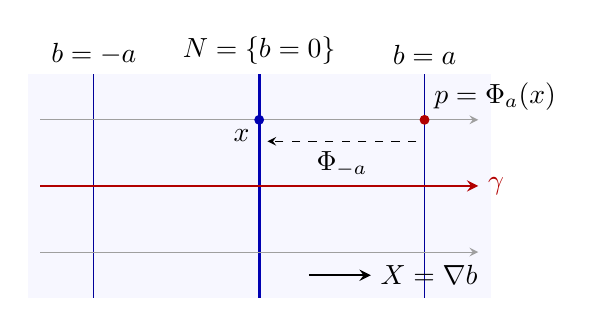
\begin{tikzpicture}[>=stealth,scale=1.05]
	\fill[blue!3] (-2.8,-1.35) rectangle (2.8,1.35);
	\draw[blue!60!black] (-2,-1.35)--(-2,1.35);
	\draw[very thick,blue!70!black] (0,-1.35)--(0,1.35);
	\draw[blue!60!black] (2,-1.35)--(2,1.35);
	\node[above] at (-2,1.35) {\(b=-a\)};
	\node[above] at (0,1.35) {\(N=\{b=0\}\)};
	\node[above] at (2,1.35) {\(b=a\)};
	\draw[->,gray!75] (-2.65,-.8)--(2.65,-.8);
	\draw[->,thick,red!70!black] (-2.65,0)--(2.65,0);
	\node[right,red!70!black] at (2.65,0) {\(\gamma\)};
	\draw[->,gray!75] (-2.65,.8)--(2.65,.8);
	\fill[blue!70!black] (0,.8) circle (1.7pt);
	\fill[red!70!black] (2,.8) circle (1.7pt);
	\node[below left] at (0,.8) {\(x\)};
	\node[above right] at (2,.8) {\(p=\Phi_a(x)\)};
	\draw[->,dashed] (1.9,.54)--(.1,.54);
	\node[below] at (1,.54) {\(\Phi_{-a}\)};
	\draw[->,thick] (.6,-1.08)--(1.35,-1.08);
	\node[right] at (1.35,-1.08) {\(X=\nabla b\)};
\end{tikzpicture}

	\caption[平行梯度流与水平集乘积]{平行梯度流把 \(N=b^{-1}(0)\) 等距地送到各水平集。点 \(p\) 的乘积坐标是 \((b(p),\Phi_{-b(p)}p)\)。图中水平箭头表示流轨道，纵向线表示水平集；它们的平面形状只用于标示相交关系。}
	\label{g3:fig:splitting-flow}
\end{figure}

\begin{example}\label{g3:exm:ray-without-line-paraboloid}
	在 \(\mathbb R^3\) 中取抛物面 \(P=\{z=x^2+y^2\}\)，带诱导度量。用 \((x,y)\) 参数表示，度量为
	\[
		g=\mathrm dx^2+\mathrm dy^2+(2x\,\mathrm dx+2y\,\mathrm dy)^2
		\ge\mathrm dx^2+\mathrm dy^2.
	\]
	因此其内在 Cauchy 列在参数平面中也 Cauchy；参数落在某个有界圆盘内时，\(g\) 又受 Euclid 度量的常数倍控制，所以 Euclid 极限也是内在极限。故 \(P\) 完备，且显然非紧。\cref{g3:lem:complete-noncompact-ray}保证它从每点都有射线。

	取上单位法向 \((-2x,-2y,1)/\sqrt{1+4x^2+4y^2}\)。相应第二基本形式是 \(2(\mathrm dx^2+\mathrm dy^2)/\sqrt{1+4x^2+4y^2}\)，而第一基本形式的行列式为 \(1+4x^2+4y^2\)。Gauss 方程因而给出
	\[
		K=\frac{\det\operatorname{Hess}(x^2+y^2)}
		{(1+|\nabla(x^2+y^2)|^2)^2}
		=\frac4{(1+4x^2+4y^2)^2}>0.
	\]
	二维中 \(\operatorname{Ric}=Kg>0\)。若它有直线，分裂定理就给出 \(P\cong\mathbb R\times N^1\)；但两个一维因子的黎曼乘积曲率为零，与上式矛盾。所以有射线与有直线确有区别。
\end{example}

分裂结论也不能直接从一个覆盖空间下降到商空间。例如 \(\mathbb R^n\) 含有许多直线并可分裂，取格点平移的商却得到紧平坦环面。覆盖投影保持测地线方程与局部长度，却可能使远处两点有更短的连接，因而不保持直线的整体最短性。章末习题还会给出非紧平坦商空间的同类现象。

\ProseParagraphBreak

完备性控制的是另一个步骤。在 \(\mathbb R^2\setminus\{(0,1)\}\) 的 Euclid 度量上，\(b(x,y)=x\) 光滑调和，\(\nabla b=\partial_x\) 平行且长为一，\(x\) 轴也是测地直线。但是从 \((-1,1)\) 出发的梯度轨道在时间一到达被删去的点，不能继续；零水平集也断成两部分。这说明上述流与逆映射的整体构造确实使用了完备性。
% 纲要条目排为编号小节标题，并进入目录与书签；说明段仍保留于纲要注释中。


\begin{chaptersummary}
	Hodge 理论以度量为每个 de Rham 类选出唯一调和代表。Green 算子的两阶正则性增益给出正合、余正合与调和的正交分解；星算子把非零调和形式变成与它积分不为零的互补次数形式，从而得到对偶。代表和 Hodge 内积随度量改变，外积积分配对则由定向与上同调类决定；不可定向情形通过定向线丛保存同一配对结构。

	\ProseParagraphBreak

	Weitzenböck 公式把调和形式的外微分能量改写为协变导数能量与曲率项。一形式上的曲率项是 Ricci 作用，高阶形式需要相应的 \(\mathcal R_q\)。非负性给出平行性，某点的正定性给出消失。离开紧情形以后，距离截断将积分问题化为环带误差；完备性、平方可积性和增长条件各自承担明确的作用。

	\ProseParagraphBreak

	分裂证明把这些工具用在一条测地直线上。两侧 Busemann 函数之和具有内部最大值，弱最大值原理使它恒为零，因而两侧函数各自调和并光滑。沿渐近射线的增长确定梯度长度为一，Bochner 公式使该梯度平行；完整的梯度流最终把流形等距地识别为水平集与实直线的乘积。
\end{chaptersummary}

\BookExercises

\begin{exercise}\label{g3:ex:self-dual-four-forms}
	在定向四维内积空间的正向正交余标架 \(e^1,e^2,e^3,e^4\) 中，求 \(*:\Lambda^2\to\Lambda^2\) 的两个特征空间及正交归一基。再设 \(M\) 为定向闭四维黎曼流形，证明每个实调和二形式唯一分为调和的自对偶与反自对偶部分，并计算 \(\int_M\omega\wedge\omega\)。
\end{exercise}
\begin{solution}
	记 \(e^{ij}=e^i\wedge e^j\)。补指标的排列符号给出
	\[
		*e^{12}=e^{34},\qquad *e^{13}=-e^{24},\qquad
		*e^{14}=e^{23}.
	\]
	因为二形式上 \(*^2=I\)，反方向的三个公式也随之确定。特征值 \(+1\) 的正交归一基为
	\[
		\frac{e^{12}+e^{34}}{\sqrt2},\quad
		\frac{e^{13}-e^{24}}{\sqrt2},\quad
		\frac{e^{14}+e^{23}}{\sqrt2};
	\]
	把每项中的第二个加数变号，便得特征值 \(-1\) 的正交归一基。两空间各三维且互相正交。

	在流形上令 \(\omega_\pm=(\omega\pm *\omega)/2\)。星与 Laplace 交换，所以 \(\omega\) 调和时两个分量都调和；特征空间分解保证唯一。由于 \(\omega_+,\omega_-\) 正交，
	\[
		\omega\wedge\omega
		=\omega_+\wedge *\omega_+
		-\omega_-\wedge *\omega_-
		=(|\omega_+|^2-|\omega_-|^2)\operatorname{vol}_g.
	\]
	于是所求积分为 \(\|\omega_+\|_2^2-\|\omega_-\|_2^2\)。中间次数的外积配对在这两个调和子空间上分别正定、负定；它与始终正定的 Hodge 内积不同。
\end{solution}

\begin{exercise}\label{g3:ex:explicit-torus-hodge-pieces}
	在标准平坦环面 \((\mathbb R/2\pi\mathbb Z)^2\) 上，对
	\[
		\omega=(2+\cos x)\,\mathrm dx+(-1+\sin x)\,\mathrm dy
	\]
	求调和、正合与余正合分量，并求 \(\delta G_1\omega\)、\(\mathrm dG_1\omega\)。计算三个分量各自的平方 \(L^2\) 范数。
\end{exercise}
\begin{solution}
	平坦环面上的调和形式系数为常数，故
	\(h=2\,\mathrm dx-\mathrm dy\)。
	其余两个分量可直接写成
	\[
		\mathrm d(\sin x)=\cos x\,\mathrm dx,\qquad
		\delta(\cos x\,\mathrm dx\wedge\mathrm dy)=\sin x\,\mathrm dy.
	\]
	二者都具有零平均系数，且它们与 \(h\) 及彼此正交，故这就是 Hodge 分解。

	Laplace 逐分量作用为 \(-\partial_x^2-\partial_y^2\)，所以
	\[
		G_1\omega=\cos x\,\mathrm dx+\sin x\,\mathrm dy,
		\qquad
		\delta G_1\omega=\sin x,\qquad
		\mathrm dG_1\omega=\cos x\,\mathrm dx\wedge\mathrm dy.
	\]
	这里 Green 解的系数均零平均，确实正交于调和核。环面面积为 \(4\pi^2\)，而 \(\int_0^{2\pi}\cos^2x\,\mathrm dx=\int_0^{2\pi}\sin^2x\,\mathrm dx=\pi\)，故三个平方范数分别为
	\(20\pi^2,2\pi^2,2\pi^2\)，总和为 \(24\pi^2\)。
\end{solution}

\begin{exercise}\label{g3:ex:conformal-middle-hodge}
	设 \(M^n\) 为定向闭黎曼流形，\(\widetilde g=e^{2\varphi}g\)，其中 \(\varphi\) 为实光滑函数。证明在 \(k\) 形式上
	\[
		*_{\widetilde g}=e^{(n-2k)\varphi}*_g.
	\]
	当 \(n=2k\) 时，证明两度量的调和 \(k\) 形式空间相同，且这些形式的 \(L^2\) 内积相同。说明这一结论为何不意味着所有次数的调和代表都不变。
\end{exercise}
\begin{solution}
	余切向量的内积乘以 \(e^{-2\varphi}\)，所以 \(k\) 形式内积乘以 \(e^{-2k\varphi}\)；体积形式乘以 \(e^{n\varphi}\)。代入星的定义，由外积配对的非退化性得到所求公式。同时
	\[
		(\alpha,\beta)_{\widetilde g}
		=\int_M e^{(n-2k)\varphi}\langle\alpha,\beta\rangle_g\,\mu_g.
	\]
	在中间次数上，这个内积不变。

	若 \(n=2k\)，内侧作用于 \(k\) 形式的星不变，而外侧作用于 \(k+1\) 形式的星乘以 \(e^{-2\varphi}\)，因此
	\(\delta_{\widetilde g}\alpha=e^{-2\varphi}\delta_g\alpha\)。
	外微分本来就与度量无关。闭流形上的调和条件等价于 \(\mathrm d\alpha=\delta\alpha=0\)，故两种调和空间相同。其他次数中，内侧星的比例因子一般不是常数，外微分会对它求导；例如正文中非恒定共形环面的调和顶次形式由常系数 \(\mathrm dx\wedge\mathrm dy\) 变成 \(e^{2\varphi}\mathrm dx\wedge\mathrm dy\) 的常数倍。
\end{solution}

\begin{exercise}\label{g3:ex:circle-pullback-projection}
	两圆周都带标准度量 \(\mathrm d\theta^2\)。给定整数 \(m\ge1\) 及 \(0<|\varepsilon|<m\)，令
	\[
		F([\theta])=[m\theta+\varepsilon\sin\theta].
	\]
	证明 \(F\) 是 \(m\) 重光滑覆盖，计算 \(F^*(\mathrm d\theta)\) 的调和代表。它本身是否调和？若将源圆周的度量改为 \(F^*(\mathrm d\theta^2)\)，答案如何变化？
\end{exercise}
\begin{solution}
	实直线上的提升 \(\widetilde F(\theta)=m\theta+\varepsilon\sin\theta\) 满足
	\(\widetilde F(\theta+2\pi)=\widetilde F(\theta)+2m\pi\)，故下降为圆周映射。其导数 \(m+\varepsilon\cos\theta>0\)，且提升严格递增、从 \(-\infty\) 走到 \(+\infty\)。在一周期内，每个模 \(2\pi\) 的值恰有 \(m\) 个原像；逆函数定理在每个原像附近给出局部光滑逆，因而是 \(m\) 重覆盖。

	拉回为
	\[
		F^*(\mathrm d\theta)
		=(m+\varepsilon\cos\theta)\,\mathrm d\theta
		=m\,\mathrm d\theta+\mathrm d(\varepsilon\sin\theta).
	\]
	标准度量下，一形式调和当且仅当系数为常数，所以它不调和，调和代表为 \(m\,\mathrm d\theta\)。新度量为 \(a^2\mathrm d\theta^2\)，其中 \(a=m+\varepsilon\cos\theta>0\)。此时拉回恰为 \(a\,\mathrm d\theta\)，由余微分公式立即得到它调和。这个局部等距的拉回现象与普通光滑拉回后需要调和投影的情形相符。
\end{solution}

\begin{exercise}\label{g3:ex:sphere-top-form-primitive}
	设 \(S^2\subset\mathbb R^3\) 为单位球面，带标准度量和外法向定向，\(z\) 为第三坐标限制。求方程
	\[
		\Delta_2 u=z\,\operatorname{vol}_{S^2}
	\]
	唯一正交于调和核的解，并为 \(z\,\operatorname{vol}_{S^2}\) 写出一个全局光滑原像。若右端改为 \((1+z)\operatorname{vol}_{S^2}\)，方程是否可解？
\end{exercise}
\begin{solution}
	球面梯度为 \(\nabla z=e_3-zx\)。沿球面切向量 \(X\) 求环境导数并取切向部分，得
	\(\nabla_X\nabla z=-zX\)，故 \(\operatorname{Hess}z=-zg\)、\(\Delta_0z=2z\)。反射对称性给出 \(\int_{S^2}z\,\mu_g=0\)。
	星与 Laplace 交换，因此
	\[
		u=\frac12z\,\operatorname{vol}_{S^2}
	\]
	满足方程。调和顶次形式是体积形式的常数倍，上述零积分保证 \(u\) 正交于它们，所以解具有所要求的唯一性。

	令 \(\eta=\delta u=-\tfrac12*\mathrm dz\)。由于 \(\mathrm du=0\)，有
	\(\mathrm d\eta=\Delta_2u=z\,\operatorname{vol}_{S^2}\)。
	它的光滑性已由整体星算子保证；在球坐标 \(z=\cos\theta\) 中还可写成
	\[
		\eta=\frac12\sin^2\theta\,\mathrm d\phi
		=\frac12(x\,\mathrm dy-y\,\mathrm dx)\big|_{S^2},
	\]
	最后一个表达式直接说明极点处没有奇性。若改用右端 \((1+z)\operatorname{vol}_{S^2}\)，它与调和体积形式的内积为 \(4\pi\ne0\)，不满足 Green 可解条件，故无解。
\end{solution}

\begin{exercise}\label{g3:ex:torus-two-pairings}
	在 \(T^2=(\mathbb R/2\pi\mathbb Z)^2\) 上取定向 \(\mathrm dx\wedge\mathrm dy\) 及度量
	\(g=a^2\mathrm dx^2+b^2\mathrm dy^2\)，其中 \(a,b>0\) 为常数。在 \(H_{\mathrm{dR}}^1(T^2;\mathbb R)\) 的基 \([\mathrm dx],[\mathrm dy]\) 中，分别计算外积积分配对、Hodge 内积及星算子的矩阵。解释前者与后两者对 \(a,b\) 的依赖为何不同。
\end{exercise}
\begin{solution}
	系数恒定的形式 \(\mathrm dx,\mathrm dy\) 调和，且由平坦环面的 Hodge 计算构成一阶上同调基。正交余标架为 \(a\,\mathrm dx,b\,\mathrm dy\)，所以
	\[
		*\mathrm dx=\frac ba\,\mathrm dy,\qquad
		*\mathrm dy=-\frac ab\,\mathrm dx.
	\]
	以输入向量的像作为矩阵列，星矩阵为
	\[
		S=\begin{pmatrix}0&-a/b\\ b/a&0\end{pmatrix}.
	\]
	积分 \(\int_{T^2}\mathrm dx\wedge\mathrm dy=4\pi^2\)，故外积配对矩阵为
	\[
		I=4\pi^2\begin{pmatrix}0&1\\-1&0\end{pmatrix}.
	\]
	Hodge 内积满足 \((\alpha,\beta)=\int\alpha\wedge *\beta\)，所以其矩阵为
	\[
		G=IS=4\pi^2\begin{pmatrix}b/a&0\\0&a/b\end{pmatrix}.
	\]
	外积积分只用定向和上同调类；度量决定互补方向的长度比例，从而改变星与正定内积。这里 \(S^2=-I_2\)，而 \(IS\) 正定，亦与一形式星的平方及配对公式一致。
\end{solution}

\begin{exercise}\label{g3:ex:ricci-eigenvalue-bound}
	设 \(M^n\) 为连通闭黎曼流形，\(n\ge2\)，且
	\(\operatorname{Ric}\ge(n-1)\kappa g\)，其中 \(\kappa>0\)。
	\begin{enumerate}
		\item 证明对任意实光滑函数 \(f\)，有
		\[
			\int_M(\Delta f)^2\,\mu_g
			=\int_M|\operatorname{Hess}f|^2\,\mu_g
			 +\int_M\operatorname{Ric}(\nabla f,\nabla f)\,\mu_g.
		\]
		\item 若 \(f\ne0\)、\(\Delta f=\lambda f\)、\(\lambda>0\)，证明
		\(\lambda\ge n\kappa\)。若取等，证明
		\(\operatorname{Hess}f=-\kappa f\,g\)。
		\item 在单位圆球 \(S^n\) 上用坐标函数验证下界达到。
	\end{enumerate}
\end{exercise}
\begin{solution}
	1. 对函数 Bochner 公式积分，左侧的散度积分为零，而
	\[
		\int_M\langle\nabla\Delta f,\nabla f\rangle\,\mu_g
		=\int_M(\Delta f)^2\,\mu_g.
	\]
	移项即得恒等式。

	2. 对称矩阵的迹不等式给出
	\[
		|\operatorname{Hess}f|^2
		\ge\frac1n(\operatorname{tr}\operatorname{Hess}f)^2
		=\frac1n(\Delta f)^2.
	\]
	又有 \(\int|\nabla f|^2=\lambda\int f^2\)。因此
	\[
		\lambda^2\int f^2
		\ge\frac{\lambda^2}{n}\int f^2
		    +(n-1)\kappa\lambda\int f^2.
	\]
	除以正数 \((n-1)\lambda\int f^2\)，得到
	\(\lambda/n\ge\kappa\)。若 \(\lambda=n\kappa\)，则上述两项非负误差的积分都为零，特别是
	\[
		\operatorname{Hess}f
		=\frac{\operatorname{tr}\operatorname{Hess}f}{n}g
		=-\frac{\lambda f}{n}g=-\kappa f\,g
	\]
	逐点成立。

	3. 在 \(S^n\subset\mathbb R^{n+1}\) 上取 \(f(x)=x_{n+1}\)，并以
	\(E=(0,\ldots,0,1)\) 表示环境常向量。切向梯度为
	\(\nabla f=E-fx\)。对切向量 \(X\) 求环境导数再投到切空间，
	\[
		\nabla_X\nabla f
		=\bigl(-X(f)x-fX\bigr)^\top=-fX.
	\]
	故 \(\operatorname{Hess}f=-fg\)，取负迹得 \(\Delta f=nf\)。
	单位圆球的 Ricci 曲率为 \((n-1)g\)，所以 \(\kappa=1\) 时下界取等。
\end{solution}

\begin{exercise}\label{g3:ex:parallel-forms-sphere-circle}
	给 \(M=S^2\times S^1\) 配单位圆球与长度 \(2\pi\) 圆周的乘积度量。记
	\(\vartheta\) 为圆周上的标准平行一形式，\(\sigma\) 为圆球的面积形式，并沿投影拉回到 \(M\)。求各阶实调和形式，证明它们分别由
	\[
		1,\qquad \vartheta,\qquad \sigma,\qquad
		\sigma\wedge\vartheta
	\]
	张成。说明这里 Ricci 非负为何没有给出一阶消失。
\end{exercise}
\begin{solution}
	乘积联络保持两个因子的分布。圆球切平面的曲率算子为一，含圆周方向的混合二向量曲率为零，所以整个曲率算子非负。因此各阶调和形式均平行。

	对调和一形式 \(\alpha\)，令 \(X=\alpha^\sharp\)。它满足
	\(\operatorname{Ric}(X,X)=0\)。乘积的 Ricci 二次型为
	\[
		\operatorname{Ric}(X,X)=|X_{S^2}|^2,
	\]
	故 \(X\) 只能沿圆周方向，\(\alpha=h\vartheta\)。
	因为 \(\alpha,\vartheta\) 都平行且 \(\vartheta\) 无零点，得到
	\(\mathrm dh=0\)，连通性给出 \(h\) 为常数。因此
	\(\mathcal H^1(M)=\mathbb R\vartheta\)。

	取乘积定向。Hodge 星保持平行性并在一形式与二形式间给出同构，而
	\(*\vartheta=\sigma\)，故 \(\mathcal H^2(M)=\mathbb R\sigma\)。
	零阶调和函数平行，因而为常数；星再给出
	\(\mathcal H^3(M)=\mathbb R(\sigma\wedge\vartheta)\)。
	这些列出的形式确实都平行，所以同时证明了包含关系的另一方向。

	Ricci 在每一点的圆周方向上都为零，因此没有任何一点使其正定。一阶形式 \(\vartheta\) 恰好处于这一零方向中。它的圆周积分为 \(2\pi\)，所以其上同调类非零。
\end{solution}

\begin{exercise}\label{g3:ex:flat-quotient-parallel-invariants}
	在 Euclid 平面上令
	\[
		a(x,y)=(x+1,y),\qquad b(x,y)=(-x,y+1),
	\]
	并令 \(\Gamma\) 为它们生成的等距变换群。证明
	\(M=\mathbb R^2/\Gamma\) 是连通闭平坦曲面，并求其全部实调和形式。由此说明平坦性不保证 \(b_1(M)=\dim M\)。
\end{exercise}
\begin{solution}
	关系 \(bab^{-1}=a^{-1}\) 说明每个群元素可唯一写成
	\(a^m b^k\)，作用为
	\[
		a^m b^k(x,y)=((-1)^k x+m,y+k),
		\qquad m,k\in\mathbb Z.
	\]
	若 \(k\ne0\)，其第二坐标发生非零平移；若 \(k=0,m\ne0\)，第一坐标发生非零平移。因此非恒等元素均无不动点。对任意紧集，只有有限个整数 \(m,k\) 能使其像与原紧集相交，所以作用适当不连续，商为光滑无边界曲面，平坦度量下降。先用 \(b\) 的幂把 \(y\) 移入 \([0,1]\)，再用 \(a\) 的幂把 \(x\) 移入 \([0,1]\)，可见紧矩形的像覆盖商空间，故商紧。连通性从 \(\mathbb R^2\) 继承。

	曲率项恒为零，所以调和形式恰为平行形式。将其提升到 \(\mathbb R^2\)，平行性意味着它在标准余标架中的系数为常数；下降的条件恰是 \(\Gamma\) 不变性。平移 \(a\) 不改变这些常系数形式，而
	\[
		b^*\mathrm dx=-\mathrm dx,\qquad
		b^*\mathrm dy=\mathrm dy,\qquad
		b^*(\mathrm dx\wedge\mathrm dy)
		   =-\mathrm dx\wedge\mathrm dy.
	\]
	故零阶调和空间为 \(\mathbb R\)，一阶由下降的 \(\mathrm dy\) 张成，二阶为零。于是
	\(b_0=1,b_1=1,b_2=0\)。平坦度量的环路平行移动仍可翻转一个方向；平行一形式必须同时保留这一信息，所以其维数可以小于二。该曲面非定向，其 Poincar\'e 配对应像式\eqref{g3:eq:twisted-poincare-pairing}那样使用定向线丛，不能要求普通实系数的零阶与顶阶维数相等。
\end{solution}

\begin{exercise}\label{g3:ex:bochner-cohomology-subalgebra}
	设 \(M^n\) 为连通闭黎曼流形。
	\begin{enumerate}
		\item 若 \(\operatorname{Ric}\ge0\)、\(r=b_1(M)\)，证明由外积诱导的分次代数映射
		\[
			\Lambda^*H_{\mathrm{dR}}^1(M;\mathbb R)
			\longrightarrow H_{\mathrm{dR}}^*(M;\mathbb R)
		\]
		为单射。因此 \(b_q(M)\ge\binom rq\)，其中 \(0\le q\le r\)。
		\item 若曲率算子 \(\mathcal R\ge0\)，证明对每个 \(p\in M\)，将上同调类先取调和代表再在 \(p\) 求值，给出分次代数单射
		\[
			H_{\mathrm{dR}}^*(M;\mathbb R)
			\longrightarrow\Lambda^*\mathrm T_p^*M.
		\]
	\end{enumerate}
\end{exercise}
\begin{solution}
	1. 取 \(H_{\mathrm{dR}}^1\) 的一组基的调和代表
	\(\alpha_1,\ldots,\alpha_r\)。Ricci 非负使它们全部平行。固定一点 \(p\)；求值映射在平行形式上单射，因此
	\(\alpha_1(p),\ldots,\alpha_r(p)\) 线性无关。相应的
	\(\binom rq\) 个外积在 \(\Lambda^q\mathrm T_p^*M\) 中线性无关。

	每个全局外积
	\(\alpha_{i_1}\wedge\cdots\wedge\alpha_{i_q}\) 都平行，因而调和。若这些形式的某个线性组合代表零上同调类，则它作为调和代表只能为零；在 \(p\) 求值，得到全部系数为零。因此每个次数上的映射均单射。外积与上同调乘法的定义相容，故所得映射是分次代数单射，并得到维数下界。

	2. 曲率算子非负使所有次数的调和形式都平行，所以两个调和形式的外积仍平行且调和。它代表两个原上同调类的乘积，故由唯一性，这个外积就是乘积类的调和代表。于是取调和代表成为分次代数同构到调和形式组成的子代数。求值显然保持外积，且在每个次数的平行形式空间上单射，复合即为所求。通常调和形式的外积未必调和；这里使乘法相容的具体原因是平行性。
\end{solution}

\begin{exercise}\label{g3:ex:incomplete-cutoff-obstruction}
	在不完备流形 \((0,1)\) 上取 Euclid 度量。证明若 \(\chi\) 紧支、Lipschitz 且 \(\chi(1/2)=1\)，则 \(\|\chi'\|_{L^\infty}\ge2\)。据此说明不能存在局部最终等于一而梯度范数趋零的紧支截断族。用 \(u(x)=x\) 检验不完备情形下 \(L^2\) 分布调和函数未必为常数，并指出对它直接使用全空间能量恒等式错在哪里。
\end{exercise}
\begin{solution}
	紧支性使某个 \(a\in(0,1/2)\) 满足 \(\chi(a)=0\)。绝对连续性给出
	\[
		1=|\chi(1/2)-\chi(a)|
		\le(1/2-a)\|\chi'\|_\infty,
	\]
	因此 \(\|\chi'\|_\infty\ge(1/2-a)^{-1}>2\)，尤其有题设下界。局部最终等于一的族必定在 \(1/2\) 处最终取值一，故梯度范数不可能趋零。

	函数 \(u=x\) 满足 \(-u''=0\) 且 \(\int_0^1u^2=1/3<\infty\)，但 \(u'=1\)。它在 \((0,1)\) 内的分布方程只允许紧支测试，不能将 \(u\) 本身直接当作紧支测试函数。若在闭区间上计算，真正的公式是
	\[
		0=\int_0^1(-u'')u
		=\int_0^1|u'|^2-[u'u]_0^1=1-1.
	\]
	被漏掉的端点通量恰好抵消梯度能量；紧支截断的导数无法趋零，反映了同一个障碍。
\end{solution}

\begin{exercise}\label{g3:ex:subquadratic-harmonic-growth}
	设 \((M,g)\) 非空、连通、完备、光滑且无边界，并有
	\(\operatorname{Vol}B_R(o)\le CR^\nu\) 对 \(R\ge1\) 成立，其中 \(\nu\ge0\)。设弱调和函数 \(u\in H^1_{\mathrm{loc}}(M;\mathbb R)\) 满足
	\[
		|u(x)-a|\le C(1+d(o,x))^\alpha
	\]
	几乎处处，其中 \(a\in\mathbb R\)、\(\alpha\ge0\)。证明若 \(2\alpha+\nu<2\)，则 \(u\) 为常数。将结论应用于平坦圆柱上的有界调和函数，并解释为什么圆柱上的非零平行一形式 \(\mathrm d\theta\) 满足式\eqref{g3:eq:harmonic-form-annular-growth}却不属于 \(L^2\)。
\end{exercise}
\begin{solution}
	在 \(A_R\) 上，增长界给出 \(|u-a|^2\le C'(1+2R)^{2\alpha}\)。所以
	\[
		R^{-2}\int_{A_R}|u-a|^2\,\mu_g
		\le C''R^{2\alpha+\nu-2}\longrightarrow0.
	\]
	\Cref{g3:prop:complete-harmonic-caccioppoli}遂给出常数结论；其连续光滑代表由\cref{g3:prop:weak-harmonic-smoothing}确定。

	在 \(S^1\times\mathbb R\) 上取 \(\mathrm d\theta^2+\mathrm dt^2\)，圆周长度为 \(2\pi\)。以 \((1,0)\) 为球心，距离球包含于 \(S^1\times(-R,R)\)，故体积至多 \(4\pi R\)。因此可取 \(\nu=1\)；有界调和函数可取 \(a=0,\alpha=0\)，满足严格不等式。

	一形式 \(\mathrm d\theta\) 的长度恒为一，平行，因而调和。其环带平方积分至多为 \(8\pi R\)，乘 \(R^{-2}\) 后趋零；但全圆柱体积无限，所以它不平方可积。这说明环带增长条件能适用于某些非 \(L^2\) 形式，而其结论只是闭、余闭或在曲率条件下平行，不能据此自动推出消失。
\end{solution}

\begin{exercise}\label{g3:ex:hyperbolic-disk-exact-l2-forms}
	在单位圆盘 \(D\subset\mathbb C\) 上取
	\[
		g=\frac{4}{(1-|z|^2)^2}(\mathrm dx^2+\mathrm dy^2).
	\]
	证明该度量完备。对整数 \(m\ge1\)，令 \(f_m(z)=\operatorname{Re}z^m\)、\(\omega_m=\mathrm df_m\)。证明 \(\omega_m\) 是非零的 \(L^2\) 调和一形式，计算 \(\|\omega_m\|_2^2\)，并证明不同 \(m\) 对应的形式两两正交。说明这些形式在普通 de Rham 上同调中的类，以及为何这不与非负曲率项下的消失结论矛盾。
\end{exercise}
\begin{solution}
	写 \(\lambda=2/(1-r^2)\)。任意从原点到半径 \(r\) 处的道路，其长度至少为
	\[
		\int_0^r\frac{2\,\mathrm ds}{1-s^2}
		=\log\frac{1+r}{1-r},
	\]
	因为沿道路有 \(|\dot r|\le|\dot z|\)；径向线段达到此长度。因此有界距离球留在 Euclid 半径严格小于一的闭盘中。该闭盘上度量与 Euclid 度量一致可比，距离闭球是紧集。Hopf--Rinow 定理给出完备性。

	二维坐标公式为
	\[
		\Delta_g f=-\lambda^{-2}(\partial_x^2f+\partial_y^2f).
	\]
	\(f_m\) 是 Euclid 调和多项式，故 \(\Delta_gf_m=0\)。于是
	\(\mathrm d\omega_m=0\)、\(\delta_g\omega_m=\Delta_gf_m=0\)，从而 \(\Delta_1\omega_m=0\)。一形式的平方长度贡献 \(\lambda^{-2}\)，密度贡献 \(\lambda^2\)，故它们相消：
	\[
		\|\omega_m\|_{L^2(g)}^2
		=\int_D|\mathrm df_m|_{\mathrm{Eucl}}^2\,\mathrm dx\mathrm dy
		=\int_0^{2\pi}\!\int_0^1m^2r^{2m-2}r\,\mathrm dr\mathrm d\theta
		=\pi m.
	\]
	对 \(m\ne\ell\)，梯度配对的角向因子为 \(\cos((m-\ell)\theta)\)，其积分为零，所以各形式两两正交。这已经给出一个无限的线性无关族。

	每个 \(\omega_m=\mathrm df_m\) 都是全局正合形式，因此其普通 de Rham 类为零；非零 \(L^2\) 调和形式不能在非紧情形中仅凭普通上同调类判定。该度量的 Gauss 曲率为负一：用 \(K=-\lambda^{-2}(\partial_x^2+\partial_y^2)\log\lambda\)，其中 \((\partial_x^2+\partial_y^2)\log\lambda=4/(1-r^2)^2\)，即可核对。二维的一形式曲率项为 Ricci 作用，故 \(\mathcal R_1=-I\)，不满足非负假设。
\end{solution}

\begin{exercise}\label{g3:ex:weak-subharmonic-limit-hypotheses}
	说明以下两点。
	\begin{enumerate}
		\item 在 \(\mathbb R^n\)、\(n\ge3\)，函数 \(u(x)=-(1+|x|^2)^{-(n-2)/2}\) 是有界、非恒定的光滑次调和函数。本书采用 \(\Delta=-\sum_i\partial_i^2\)，请计算其 \(\Delta u\) 并解释它为何不违背强最大值原理。
		\item 在 \(\mathbb R\) 上，将零函数仅在原点改成取值一。所得点态函数与零函数代表同一个 \(H^1_{\mathrm{loc}}\) 元素，且分布调和，却在原点有严格最大值。解释强最大值定理为什么要指定连续代表。
	\end{enumerate}
\end{exercise}
\begin{solution}
	（1）令 \(r=|x|\)、\(a=(n-2)/2\)。对 \(v=(1+r^2)^{-a}\)，径向求导给出
	\[
		v''+\frac{n-1}{r}v'
		=-n(n-2)(1+r^2)^{-(n+2)/2}.
	\]
	此式在原点按光滑延拓理解。由于 \(u=-v\)，有
	\[
		\Delta u=-n(n-2)(1+|x|^2)^{-(n+2)/2}<0.
	\]
	所以 \(u\) 次调和，取值于 \([-1,0)\)，而上确界零仅在趋向无穷远时逼近，没有在内部达到。强最大值原理的接触假设不满足。

	（2）改变零测集上的取值不改变任何测试积分或弱导数，所以这个点态函数的分布 Laplace 仍为零。其唯一连续调和代表是处处为零的函数，而所给的特殊点态代表不连续。强最大值结论比较的是指定连续代表的点值；若允许任意修改零测集上的值，内部极值就不再由弱方程决定。
\end{solution}

\begin{optionalexercise}\label{g3:ex:hyperbolic-busemann-failure}
	在双曲上半平面 \(\mathbb H^2=\{(x,y):y>0\}\) 上取度量 \(g=y^{-2}(\mathrm dx^2+\mathrm dy^2)\) 与直线 \(\gamma(t)=(0,e^t)\)。采用本书的 Busemann 符号与 \(\Delta=-\operatorname{div}\nabla\)。计算 \(b_+,b_-\) 及 \(\Delta b_\pm\)，验证 \(b_++b_-\le0\) 在线上取等号，却不恒为零，并指出分裂证明中的哪一项假设失效。计算中可以使用上半平面反演的等距性，但须核对它。
\end{optionalexercise}
\begin{solution}
	任意连接两点的曲线满足
	\[
		L_g(c)\ge\int\frac{|y'|}{y}\,\mathrm ds
		\ge|\log y_1-\log y_0|.
	\]
	竖直曲线达到这个下界，所以 \(\gamma\) 确为单位速直线。固定 \((x,y)\)，当 \(T>\log y\) 时，先沿竖直方向走到 \((x,e^T)\)，再水平走到 \((0,e^T)\)，得到
	\[
		T-\log y\le d_g((x,y),\gamma(T))
		\le T-\log y+|x|e^{-T}.
	\]
	因此 \(b_+(x,y)=\log y\)。

	令
	\[
		I(x,y)=\left(-\frac{x}{x^2+y^2},\frac{y}{x^2+y^2}\right).
	\]
	写成复变量就是 \(I(z)=-1/z\)，故 Euclid 长度被乘以 \(|z|^{-2}\)，新高度也等于 \(y|z|^{-2}\)，两者之比不变。因此 \(I^*g=g\)。它又满足 \(I(\gamma(-T))=\gamma(T)\)，所以
	\[
		b_-(x,y)=b_+(I(x,y))
		=\log\frac{y}{x^2+y^2}.
	\]
	于是
	\[
		b_++b_-=
		\log\frac{y^2}{x^2+y^2}\le0,
	\]
	等号恰在 \(x=0\) 时成立。

	二维共形度量的散度坐标式直接给出
	\(\Delta=-y^2(\partial_x^2+\partial_y^2)\)。从而 \(\Delta\log y=1\)；\(\log(x^2+y^2)\) 在上半平面是 Euclid 调和函数，也可由等距性得 \(\Delta b_-=1\)。所以
	\[
		\Delta(b_++b_-)=2>0.
	\]
	这里和函数是本书符号下的弱超调和函数，不能对它使用弱次调和的强最大值原理。双曲度量有 \(K=-1\)，从而 \(\operatorname{Ric}=-g\)；失效的正是 Ricci 非负条件，而直线与完备性均成立。
\end{solution}

\begin{optionalexercise}\label{g3:ex:flat-mobius-no-line}
	令 \(G:\mathbb R^2\to\mathbb R^2\) 为 \(G(x,y)=(x+1,-y)\)，并给商空间
	\[
		M=\mathbb R^2/\langle G\rangle
	\]
	赋予使投影局部等距的平坦度量。证明 \(M\) 光滑、无边界、完备且非紧，并显式给出一条射线；再证明 \(M\) 没有测地直线。由此说明在非紧情形，万有覆盖中的等距 \(\mathbb R\) 因子也可能不能下降到商空间。
\end{optionalexercise}
\begin{solution}
	有 \(G^k(x,y)=(x+k,(-1)^ky)\)。非零整数 \(k\) 改变 \(x\) 坐标，所以作用自由；对两个固定紧集，只有有限个整数平移能使其相交。因此作用适当不连续。每个半径小于 \(1/3\) 的 Euclid 小球与其非平凡平移不交，投影在这样的球上给出局部等距坐标，于是商是光滑无边界平坦流形。

	Euclid 覆盖空间完备，\cref{g3:prop:riemannian-covering-distance}给出商的完备性及距离公式
	\[
		d_M([p],[q])=\min_{k\in\mathbb Z}|p-G^kq|.
	\]
	函数 \(|y|\) 下降到商上且无界，故 \(M\) 非紧。曲线 \(\eta(t)=[(0,t)]\)、\(t\ge0\)，是一条射线：对 \(s,t\ge0\)，偶数 \(k\) 给出的距离平方是 \(k^2+(s-t)^2\)，奇数 \(k\) 给出 \(k^2+(s+t)^2\)。它们均不小于 \((s-t)^2\)，且 \(k=0\) 达到该值。

	另一方面，商上的任意单位速全时测地线都能提升为 Euclid 单位速直线
	\[
		\widetilde\sigma(t)=(at+b,ct+d),\qquad a^2+c^2=1.
	\]
	对任意 \(T>0\)，选奇数 \(k_T\) 使 \(|2aT+k_T|\le1\)。则
	\[
		\bigl|\widetilde\sigma(-T)-G^{k_T}\widetilde\sigma(T)\bigr|^2
		=(2aT+k_T)^2+4d^2\le1+4d^2.
	\]
	因此其投影两端的距离有与 \(T\) 无关的上界，而参数长度为 \(2T\)。充分大的 \(T\) 使该段不再最短，所以不存在测地直线。任意 \(\mathbb R\times N\) 都含有直线，故 \(M\) 不可能有这样的整体等距分解，尽管其万有覆盖就是可分裂的 \(\mathbb R^2\)。
\end{solution}

\begin{optionalexercise}\label{g3:ex:several-harmonic-functions-splitting}
	设 \((M^n,g)\) 连通、完备、光滑、无边界且 \(\operatorname{Ric}\ge0\)。设 \(1\le k\le n\)，\(f_1,\ldots,f_k\) 为实值光滑调和函数，满足 \(\sum_{i=1}^k|\nabla f_i|^2\) 为常数，并且 \((\nabla f_i)\) 在某一点线性无关。证明 \(M\) 等距于 \(\mathbb R^k\times N\)，其中 \(N\) 连通完备且具有非负 Ricci 曲率。说明为什么只假定存在 \(k\) 个线性无关的平行向量场还不足以得到这个结论。
\end{optionalexercise}
\begin{solution}
	对每个 \(f_i\) 使用函数 Bochner 公式并求和。总梯度平方为常数，调和性又消去 \(\nabla\Delta f_i\)，得到
	\[
		0=-\sum_i|\operatorname{Hess}f_i|^2
		-\sum_i\operatorname{Ric}(\nabla f_i,\nabla f_i).
	\]
	每个被减去的量都非负，故每个 \(X_i=\nabla f_i\) 平行。Gram 矩阵 \(C=(\langle X_i,X_j\rangle)\) 因而在连通的 \(M\) 上恒定；一点处的线性无关使它正定。对函数向量施加常矩阵 \(C^{-1/2}\)，再减去某一点的函数值，可得到函数 \(u_1,\ldots,u_k\)，其梯度 \(Y_i\) 处处正交归一，且有共同零点。

	每个 \(Y_i\) 都有全时等距流 \(\Phi^{(i)}\)：长度为一与完备性保证全时存在，平行性保证保持度量。又有
	\[
		[Y_i,Y_j]=\nabla_{Y_i}Y_j-\nabla_{Y_j}Y_i=0.
	\]
	沿第 \(i\) 个流推前 \(Y_j\) 时向量场保持不变，积分曲线唯一性遂使这些流两两交换。由于 \(\mathrm du_j(Y_i)=\delta_{ij}\)，共同水平集
	\(N=\{u_1=\cdots=u_k=0\}\) 是非空的光滑余维 \(k\) 子流形。定义
	\[
		F(t,x)=\Phi_{t_1}^{(1)}\circ\cdots\circ\Phi_{t_k}^{(k)}(x).
	\]
	它满足 \(u_i(F(t,x))=t_i\)，而逆映射为
	\[
		p\longmapsto\left(
		(u_1(p),\ldots,u_k(p)),\,
		\Phi_{-u_1(p)}^{(1)}\circ\cdots\circ
		\Phi_{-u_k(p)}^{(k)}(p)\right).
	\]
	两式光滑且互逆，给出全局微分同胚。各个流等距并保持 \(Y_i\)，而 \(TN\) 是它们的共同正交补，所以
	\[
		g(\mathrm dF(a,v),\mathrm dF(c,w))
		=\sum_{i=1}^k a_ic_i+g_N(v,w).
	\]
	于是 \(F\) 等距。逆映射的第二分量是从连通 \(M\) 到 \(N\) 的满射，故 \(N\) 连通。\(N\) 是闭水平集；乘积投影不增加长度，因此其内在距离等于 \(M\) 距离的限制，完备性随之得到。乘积曲率公式给出 \(\operatorname{Ric}_N\ge0\)。若 \(k=n\)，连通的零维 \(N\) 就是一个点。

	平坦环面有 \(n\) 个线性无关的平行向量场，却不能等距于 \(\mathbb R^n\)。它们的对偶一形式有非零周期，并非全局实值函数的微分；本题给定的 \(f_i\) 排除了这个整体障碍。
\end{solution}

\begin{optionalexercise}\label{g3:ex:two-ends-splitting}
	设 \((M^n,g)\) 连通、完备、光滑、无边界且 \(\operatorname{Ric}\ge0\)。若存在紧集 \(K\subset M\)，使 \(M\setminus K\) 至少有两个无界连通分支，证明 \(M\) 等距于 \(\mathbb R\times N\)，其中 \(N\) 紧。提示：先连接不同分支中趋于无穷远的点，并把最短测地线经过 \(K\) 的时刻移到零。
\end{optionalexercise}
\begin{solution}
	固定 \(o\in M\)，在两个无界分支 \(U,V\) 中分别取 \(p_j,q_j\)，使 \(d(o,p_j),d(o,q_j)\to\infty\)。由完备性，存在连接 \(p_j,q_j\) 的单位速最短测地线。它必须经过 \(K\)：否则其连通像将包含在 \(M\setminus K\) 的同一个连通分支中，不能连接 \(U\) 与 \(V\)。取一个交点 \(z_j\in K\)，以此为参数零点，将曲线记为
	\[
		\sigma_j:[-a_j,b_j]\to M,
		\qquad \sigma_j(0)=z_j.
	\]
	若 \(C=\max_{z\in K}d(o,z)\)，则
	\[
		a_j=d(p_j,z_j)\ge d(o,p_j)-C\to\infty,
		\qquad b_j\to\infty.
	\]
	紧集 \(K\) 上的单位切球丛是紧的，可用有限个局部正交标架与单位球面的紧性验证。取子列使 \((z_j,\dot\sigma_j(0))\to(z,v)\)。完备性与测地线初值的光滑依赖给出全时极限测地线 \(\sigma\)。任意固定有限参数段最终包含于 \([-a_j,b_j]\)，距离的连续性使该段在极限中仍最短。因此 \(\sigma\) 是直线，分裂定理给出 \(M\cong\mathbb R\times N\)，其中 \(N\) 连通完备。

	若 \(N\) 非紧，证明 \(\mathbb R\times N\) 不可能具有题设性质。将 \(K\) 置于一个紧矩形 \([-A,A]\times C\) 内，其中 \(C\subset N\) 为紧集。非紧性保证 \(N\setminus C\ne\varnothing\)。矩形外部
	\[
		W=\bigl(((-\infty,-A)\cup(A,\infty))\times N\bigr)
		\ \cup\ \bigl(\mathbb R\times(N\setminus C)\bigr)
	\]
	是道路连通的：上下两个区域各自道路连通，因为连通流形 \(N\) 道路连通；取一个 \(x_0\in N\setminus C\)，竖直线 \(\mathbb R\times\{x_0\}\) 将它们相连；其余竖直通道也与这两个区域相交。又有 \(W\subset M\setminus K\)。题设的两个无界分支都必须与 \(W\) 相交，因为紧矩形有界。因此它们属于同一个连通分支，矛盾。故 \(N\) 必紧。
\end{solution}
